\chapter{Measurement of \bmumu Branching Fractions}
\label{sec:BFanalysis}
This Chapter presents the measurements of the \bdmumu and \bsmumu branching fractions. Section X gives an overview of the analysis strategy and a detailed description of how the number for \bmumu decays is extracted from the data is given in Section Y. The noramlisation proceedure to convert the number of observed \bmumu decays in to the branching fractions for these decays is explained in Section X and the results are given in Section Y. 

The work presented in this Chapter was performed by the \bmumu LHCb analysis group and is published here~\cite{}. My contribution was providing the ROOT files which contained the data and simulated events necessary for the analysis development and results.

\section{Analysis Strategy} 
\label{sec:BFAnalysisStrategy}

The branching fraction of \bmumu decays is the ratio of the number of \bmumu decays and the total number of \bsd mesons produced. However no detector is perfect therefore the number of observed \bmumu decays is reduced by the detection efficiency, $\epsilon$, leading to
\begin{equation}
\mathcal{B}(B^{0}_{(s)} \to \mu^{+} \mu^{-}) = \frac{\mathcal{N}(B^{0}{(s)} \to \mu^{+} \mu^{-})}{\mathcal{N}(B^{0}_{(s)})} = \frac{N^{obs}(B^{0}_{(s)} \to \mu^{+} \mu^{-})}{\mathcal{N}(B^{0}_{(s)})}
\label{eq:BFdef}
\end{equation}



%\begin{align}

%\mathcal{B}(\bmumu) = \frac{\mathcal{N}(\bmumu)}{\mathcal{N}(\bsd)} = \frac{\mathcal{N}_{obs}(\bmumu)}{\epsilon \mathcal{N}(\bsd)}
%\begin{align}

  where ...$\sigma_{\bbbar}$

The number of \bsd created is needed, this can be calculated from the integrated luminoscity, $\mathcal{L}_{int}$, and the \bbbar production cross-section, $\sigma_{\bbbar}$, by

%\begin{equation}

%\mathcal{N}(\bsd) = 2 \times \mathcal{L}_{int} \times \sigma_{\bbbar} \times f_{x}

%\end{equation}
\begin{equation}
\mathcal{N}(B^{0}_{(s)}) = 2 \times \mathcal{L}_{int} \times \sigma_{b \bar{b}} \times f_{x} 
\label{eq:NumberB}
\end{equation}

where $f_{x}$ is the hadronisation factor giving the probability for a $b$ or $\bar{b}$ quark to form a \bs or a $\bar{\bs}$ (equivently for the \bd). The factor of 2 arises because no distinction is made between the \bs and the $\bar{\bs}$. {\it should maybe reference the LHCb experiment and such like things in the detection efficiency and I need to think of a consistent way to display the Bs and Bd modes.}

Although the number of \bsd can be computed this way the unceratinies on the measured cross-section are quite large (the measured cross-section is not precisely known) as well as the hadronisation factors. Therefore to acheive a more precise branching fraction measurement an alternative approach is used where another decay with a well know branching fraction is used to normalise the number of \bmumu decays observed to obtain the branching fractions. The extraction of $\mathcal{B}$(\bmumu) from the number of observed events is done by

\begin{eqnarray}
\mathcal{B}(B^{0}_{(s)} \to \mu^{+} \mu^{-}) &=& \frac{1}{\mathcal{B}_{norm}} \cdot \frac{f_{norm}}{f_{d(s)}} \cdot \frac{\epsilon_{norm}}{\epsilon_{B^{0}_{(s)} \to \mu^{+} \mu^{-}}} \cdot \frac{\mathcal{N}_{obs}(B^{0}_{(s)} \to \mu^{+} \mu^{-})}{\mathcal{N}^{obs}_{norm}} \\
&=& \alpha_{s} \cdot \mathcal{N}_{obs}(B^{0}_{(s)} \to \mu^{+} \mu^{-})
\label{eq:BFnorm}
\end{eqnarray}

where norm. inidicates the normalisation channel, the normalisation parameters can be combined into one normalisation parameter $\alpha$ for the \bs and the \bd. The normalisation proceedure removes the uncertainty from $\sigma_{\bbbar}$ but the hadronisation factors are still included. The ratio of efficiencies also removes the dependance on simulated decays. 

Therefore the number of observed \bmumu decay and the normalisation paramters need to be determined to measure the branching fraction. The selection described in Chapter X allows \bmumu candidates to be classified by dimuon invariant mass and the BDT output. {\it mabye BDT vs mass plot?} A simultaneous unbinned maximum likelihood fit is performed to the dimuon invariant mass distribution in 4 BDT bins to measure the observed number of \bdmumu and \bsmumu decays. The Run 1 and Run 2 data are kept seperate and the fit is applied simulatanrously to both data sets. To measure the number of \bmumu decays the fit requires knowledge of the mass shapes and the fraction of decays in each BDT bin for the both \bmumu decays and the backgrounds still present in the data set. The mass and BDT probability distribution functions ($pdfs$) are described in Section X.
The binning choice used for the BDT is chosen to optimise both fit stability and senesitivity to the \bmumu branching fractions. The bin boundaries used are


\begin{equation}
[0.25, 0.4, 0.5, 0.6, 1.0].
\label{eq:BDTbins}
\end{equation}
Candidates with BDT values between 0 and 0.25 are not included in the fit because this bin is dominated by backgrounds from combinatorial decays, inclusion of this bin in the fit does not improve the branching fraction sensitivity and reduced the stability of the fit. The highest BDT is the largest due to the excellent performance of the BDT at removing background decays. Table/Figure X, shows the number of \bmumu candidates in data passing the selection described in Chapter X with dimuon mass greater that 5447 \mevcc. At high BDT values there are very few candidated therefore a wide bin is used for high BDT values to ensure there are enough candidates in high mass regions to ensure a stable, accurate fit.

The normalisation decay can be chosen to be as similar as possible to \bmumu decays to reduce systematic uncertainties caused by different detection and selection efficiencies, also it needs to be abundant so the the precision of the branching fraction measurement in not limited by the statisitic avaliable for the normalisation channel and the noralisation decay must have a precisely meased branching fraction which is likely for abundant decays. Two decays are chose as normalisation channels; \bujpsik and \bdkpi. Both decays have large, precisely measured branching fractions and are similar to \bmumu decays in complmentary ways. For \bujpsik, the trigger efficiency is very similar to \bmumu due to the two muons from the \jpsi but the extra particle, $K^{+}$ in the final state will lead to different efficiencies in the selection and reconstruction. Alternatively \bdkpi has a very similar topology to \bmumu therefore the selection and reconstruction efficincies will be similar but the trigger efficiencies for hadrons is quite different compared to muons.  

The normalisation factors $\alpha_{(s)}$ are evaluated independantly for each noramlisation channel and year of data taking, the factors are combined to produce an overall normalisation factor for Run 1 and Run 2. The computation of the normalisation factors is described in Section X. 
{\it Explain in the normalisation section that ideally a Bs decay would be best but that was not to be.}

{\it Prehaps the information about the BDT bins could go here? Some discussion should because the binning choice is used in the following sections.}

\section{Signal PDFs}
\label{sec:signalPdfs}

To measure the number of \bdmumu and \bsmumu decays the mass PDFs and fraction of both decays in each BDT bin must be know for Run 1 and Run 2 data.

\subsetion{Mass PDFs}
The mass PDFs for \bdmumu and \bsmumu decays ared modelled by a Crystal Ball function. A Crystal Ball function is a Gaussian function that has an exponential tail on the low mass sied to model radiative energy loss in the the final state. The parameters defininh the function are the mean, $\mu$, and resolution, $\sigma$ of the Gaussian, the slope of the exponetial, $n$, and a parameter $\alpha$ that determines the tracnsition point between the Gaussian and the exponeitla function that is defined in terms of $\sigma$. 

The parameters are evaluated seperatly for the \bs and the \bd from different sources:
\begin{itemize}
\item $\mu$ - the mean for \bs and \bd is evaluated from a fit to \bskk and \bdkpi decays in data
\item $\sigma$ - the resolution is extraplotaied from the resolutions of quarkonia resonances. The resolutions for the \jpsi, $\Psi (2S)$ and $\Upsilon(1, 2, 3S)$ decayin in to two muons is measure from a fit to data. The \bs and \bd resolutions are then extraploated from the observed realationship between quarkonia mass and resolution.
\item $n$ and $\alpha$ - these parameters are evaluated from the mass sepectrum of \bsmumu and \bdmumu simulated decays, the mass distribution is smeared to have the same resolution as that measured from the quarkonia decays in data.
\end{itemize}

All parameter are evaluted seperatly for teh \bd and the \bs for each year of data taking. The resulting parameter vales are in good agreement accross each of the Run 1 and Run 2 data sets. The weighted average of the yearly parameters is used to produced the msas PDFs for Run 1 and Run 2. The parameters used are given in Table~\ref{}(?).



\subsection{BDT PDFs}
%The fraction of \bmumu decays in each BDT bin is meeded to measure the branching fraction therefore the BDT PDF needs to be evaluated. 
A uniform distribution for \bmumu decyas is expected acorss the full BDT range as designed by the BDT flattening proceedure descriebd in Section~\ref{}. Therefore the fraction of \bmumu decays in a BDT bin should simply be proportional to the bin with. However to avoid any differences between simulated decays and data affecting the expected fraction of \bmumu decays in each BDT bin, the PDF of the BDT is evaluated from data, this process is know as the BDT callibration.
The global BDT is designed to used only kinematic and goemetric information to classigy candidates and include no PID information. Therefore the BDT distribution of \bhh decays, that are topologically simimlar to \bmumu decays, will have the same BDT PDF as \bmumu decays. The \bdkpi decay is used to callibrate the BDT response because it is the most abundant \bhh decay. 

The number of \bdkpi decay is extracted from data using maimum likelihood fits in each BDT bin in each year of data taking. The \bdkpi candidates must pass the standard \bhh selection in Table~\ref{} and are seperated from other \bhh modes using DLL(K-$\pi$) variable. 

The PID and trigger efficiencies are different for \bdkpi decays compared to \bmumu. Therefore the \bdkpi yields in each BDT bin are corrected for in the final PDFs. Also to reduce the difference in the trigger efficiency between \bdkip and \bmumu decays, \bdkpi candidates are required to be triggerd by TIS at the L0 and Hlt1 levels but TOS requirements are used at the Hlt2 level to ensure enough statistics.

The same callibration is used for \bsmumu and \bdmumu decays because the selection efficiencies are extremely similar. 

The callibration is preformed for each year seperately then combined to ive the Run 1 and Run 2 fractions per BDT bin. Figure~\ref{fig:BDTPDFs} shows the BDT distribution for \bsmumu calibrated with \bdkpi data for Run 1 and Run 2. 
{\it Be consistent with the use of fraction and PDF.}

\begin{figure}[htbp]
    \centering
   \begin{subfigure}[b]{0.48\textwidth}
        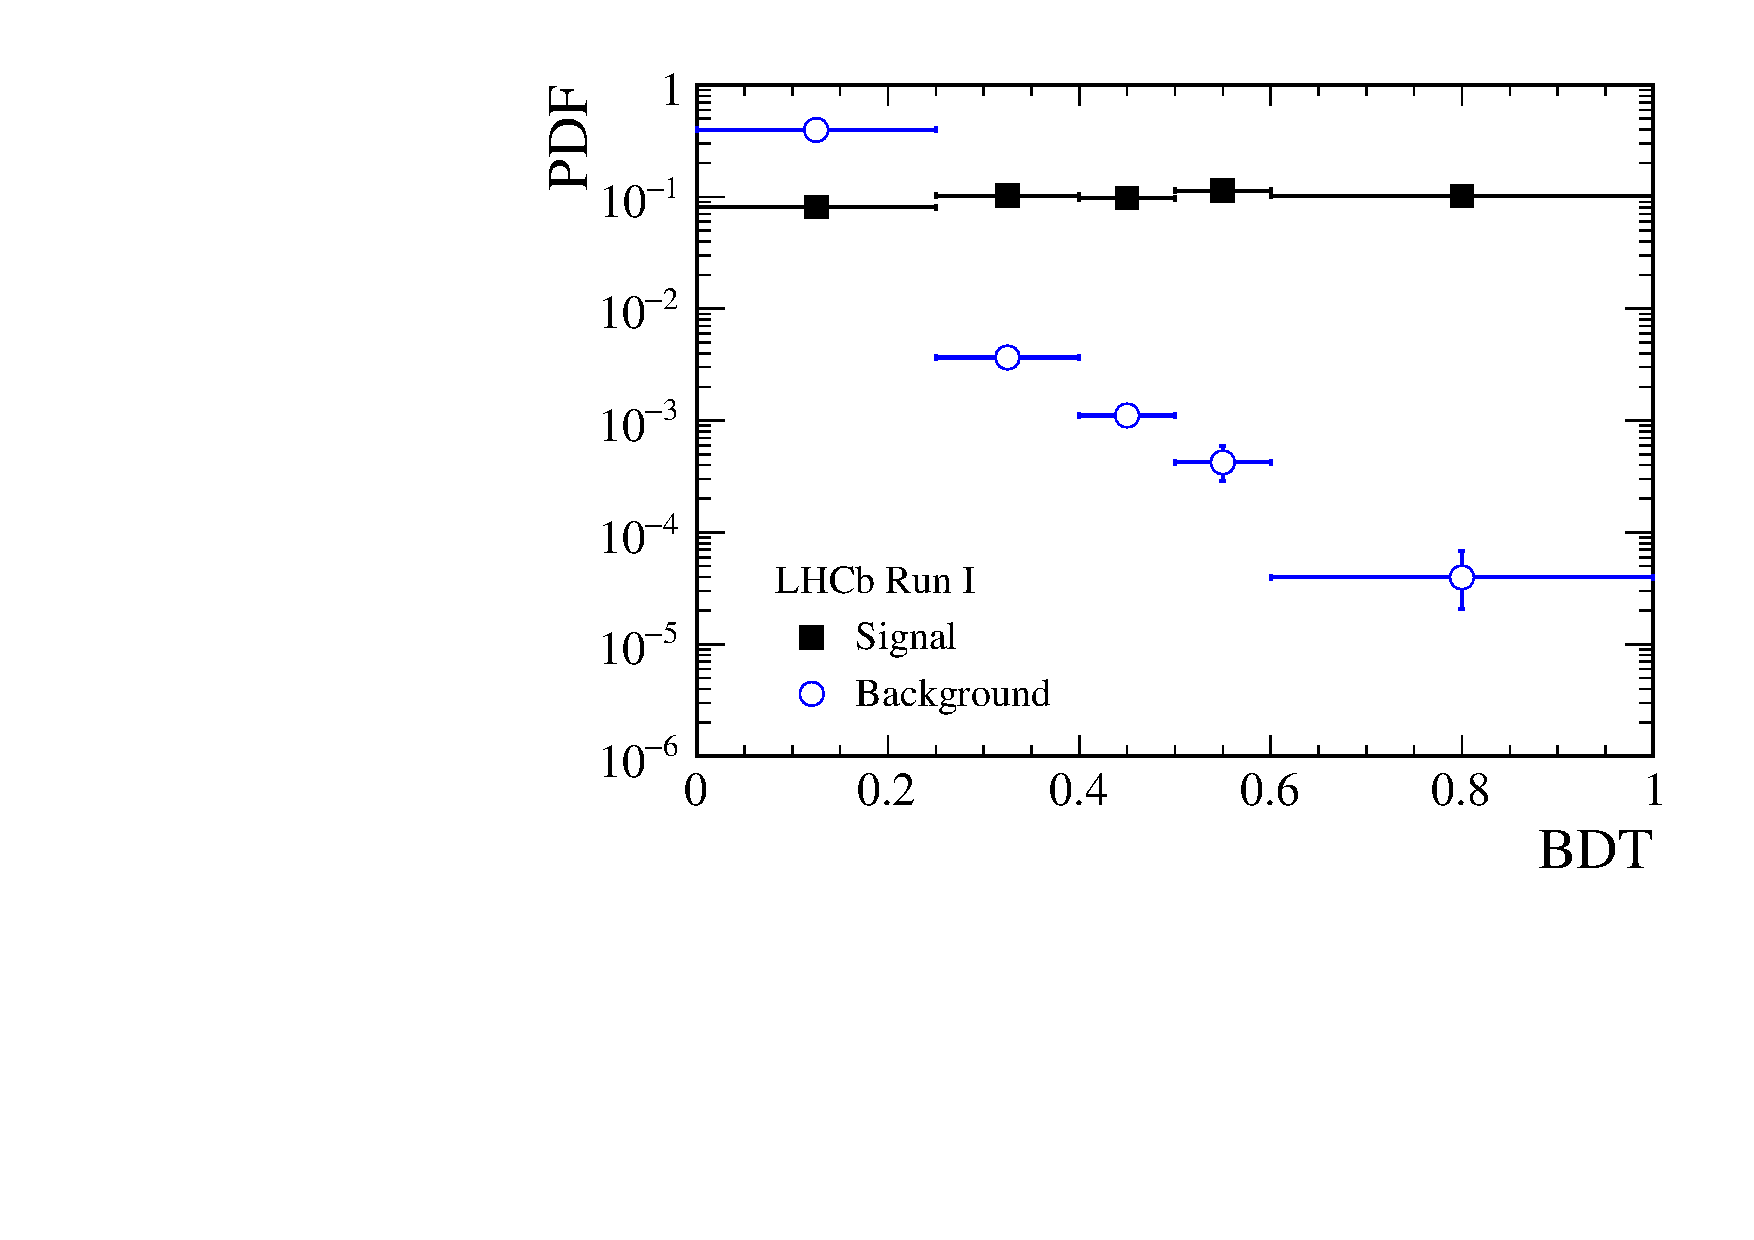
\includegraphics[width= \textwidth]{./Figs/BFAnalysis/C_macros/BDT_calibration_Run1.pdf}
        %\caption{ }
       % \label{fig:BDTSsig}
    \end{subfigure}
   % ~ %add desired spacing between images, e. g. ~, \quad, \qquad, \hfill etc. 
      %(or a blank line to force the subfigure onto a new line)
    \begin{subfigure}[b]{0.48\textwidth}
       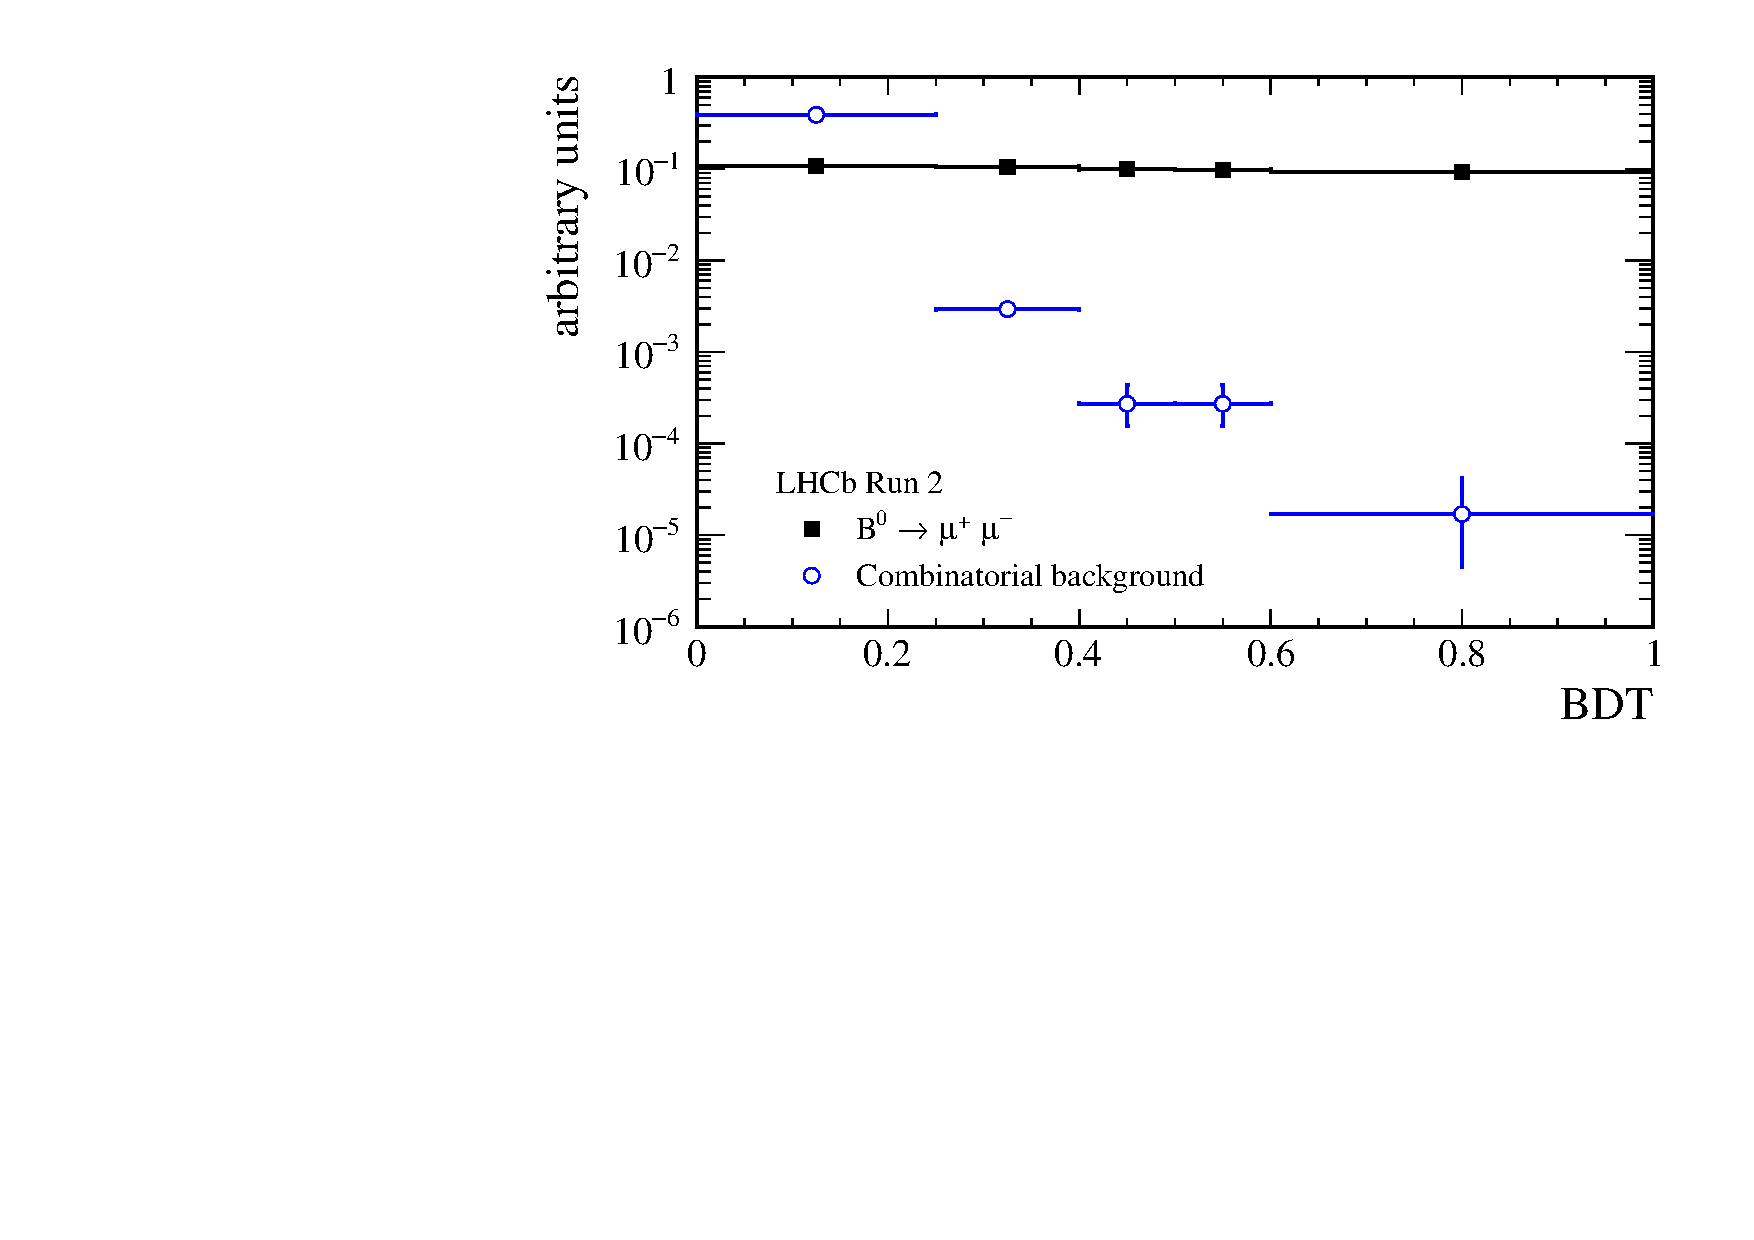
\includegraphics[width=\textwidth]{./Figs/BFAnalysis/C_macros/BDT_calibration_Run2.pdf}
      %  \caption{ }
     %   \label{fig:BDTSbkg}
   \end{subfigure}
    \caption{\bmumu BDT PDFs for Run 1 and Run 2 data callibrated on \bdkpi decay in black and the combinatorail background decays in blue for \bmumu candidates in data with a dimuon mass above 5477 \mevcc. }
    \label{fig:BDTPDFs}
\end{figure}


\subsection{Decay time dependance of BDT PDF}
The output of the gloabl BDT for \bmumu is correlated with the \bmumu decay time dur the the input variables used int eh BDT defined in SEction~\ref{}. The leads to corrections being needed for the \bsmumu BDT PDF. In the SM the \bsmumu effective lifetime, \tmumu, is equal to the lifetime of the heavy \bs mass eigenstate, \tH, however in reality \tmumu could be somewhere in between the lifetimes of the heavy and light mass eignenstates. As described in {\it the Theory Chapter} the \bsmumu effective lifetime is related to the parameter \ADG where \ADG = -1 for \tmumu = \tL and \ADG = +1 for \tmumu = \tH.

The simulated decays used to train and flatten the gloabl BDT use as the \bsmumu effective lifetime the mean of the measured \tH and \tL values at the time of production. Therefore the lifetiem used is different between simulateion versions. Since the BDT output is correlated with the lifetime the BDT PDF, the fractions of \bsmumu decays in each BDT bin, will depend on the lifetime used in teh simulation. Therefore numerical correction factor are computed for each year to scale the BDT PDF for the situation where \ADF = -1, 0 or +1. 

The final resuilts is computed assuming the SM value of \ADG = +1 but the change in cetnral value is calculated for \ADG = -1 and 0. No corrections are needed for \bdmumu becayse the decay width is negliable and the need for correction canles out wit the BDT callibration using \bdkpi. 

{\it I have some questions about this part, how are these corrections actually used since the BDT is flattened for Run 1 with 2011 and for Run 2 with 2015 MC.How is the callibration ok since it uses the B0 which has the same correlations which is this not taken into accout? Prehaps make this briefer?}

\section{Background PDFs}
\label{sec:backgrounds}
The seleciton described in Chapter X is effective at reducing the background in the data set to a suitable level so that properties of the \bmumu decays can be measured. However background decays are present in the final data set, they cannot be completly removed without drastically reducing the efficiency to select signal decays. The backgroudsn presnt in the final data set must be included in the fit to the dimuon invarianet mass in order to acuraltely measure the \bmumu branching fractions. The backgrounds are;
\begin{itemize}
\item \bhh, where h = $K$, $\pi$, when both hadrons are mis-identified as muons as they decay during their fligh through the detetor after they have left the VELO. This background falls within the \bd mass window but not the \bs mass window\footnote{\bd and \bs mass windows are defined as $\pm$ 60 \mevcc of the \bd and \bs masses.} due to the missing energy from the undetected neutrino. 
\item semi-leptonic decays where one hadron is mis-identified as a muon;
\begin{itemize}
\item \bdpimunu and \bsKmunu where the final state hadrons are mis-identified as muons. The mass of these backgrounds falls below the \bd mass window in the left mass sideband
\item \lambdab when the proton is mis-identified as a muon. The large mass of the $\Lambda_{d}$ meases that this background pollutes the \bs and \bd mass windows and the low mass sideband
\end{itemize}
\item semi-leptonic decays where muon muons in the decay form a good vertex;
\begin{itemize}
\item \bpimumu where the pion is not detected. The missing hadron means that these backgrounds fall well below the \bd mass window.
\item \bcjpsimunu where \jpsimumu. The large mass of the $B^{+}_{c}$ causes this background of cover the full mass window
\end{itemize}
\item combinatorial background from the random combination of any two muons in the event are distributed accross the full mass range
\end{itemize}

To measure the number of \bsmumu decays these backgrounds must be modelled  in the invariant mass fit in each BDT bin, therefore the mass PDFs and fraction of events present in each BDT bin must be determined.  Backgrounds that fall below the \bd and \bs mass windows still need to be accruatly modelled so that the number of combinatorial background decays that cover the full mass range can be accuratley described/measured. The proceedure is slightly different for \bhh decays compared to semi-leptonic decays.

\subsection{\bhh mass and BDT PDFs}
The mass pdf describing mis-identified \bhh decays is formed of two Crystal Ball functions. The parameter values are evaluted from simulated decays for \bdkpi, \bskk, \bdpipi and \bsKpi the have the momentum of tracks smeared to model the hadron decaying in flight. The parameters are evaluted seperately for each decay and combined using the branching fractions and the particle identification efficiencies for each decay.

The number of mis-identified \bhh decays in each BDT bin is computed from \bdkpi decays in data passing the same selection as the signal BDT callibration sample using the equation

\begin{equation}
\mathcal{N}_{B \to hh \to \mu^{+} \mu^{-}} = \epsilon^{TRIG|SEL}_{B^{0}_{(s)} \to \mu^{+} \mu^{-}} \cdot \frac{\mathcal{N}_{hh}}{\epsilon^{TRIG}} \cdot \epsilon_{hh\to \mu\mu}  \\
\label{eq:bhhprediction}
\end{equation}

The probability of a \bhh decay passing the \bmumu particle identification requirements is given by  and   is the number of \bhh decays in data determined from \bdkpi decays and scaled for the relative fraction of the total \bhh decays. The efficiency of the \bmumu triggers is given by and  is the efficiency TIS triggers used to select \bdkpi decays. The trigger and particle identification efficiencies are computed per BDT bin and the BDT pdf before the PID efficiencies is assumed to be the same as the signal PDF. 

{\it This is poor and needs re-wording when I am less tired, but I have to power on for now or this will NEVER end!}

\subsection{Semi-leptonic mass and BDT PDFs}

The mass PDFs for each semi-leptonic background are taken from fitting simualted decays for each background in BDT bins. An Argus function is used to describe the mass distributions. The shapes of \bdpimunu and \bsKmunu are extremely similar and therefore these backgrounds are modelled with one commmon PDF. Similarly one mass PDF is used to model \bpimumu decays.

The expected number of semi-leptonic backgrounds in each BDT bin is estimated by normalising to the number of \bujpsik decays observed via

\begin{eqnarray}
\mathcal{N}^{exp}_{x} &=& \mathcal{N}_{B^{+} \to J/\psi K{+}} \cdot \frac{f_{x}}{f_{u}} \cdot \frac{\mathcal{B}_{x}}{\mathcal{B}_{B^{+} \to J/\psi K^{+}}} \cdot \frac{\epsilon^{tot}_{x}}{\epsilon_{tot}^{B^{+} \to J/\psi K^{+}}} \\
&=& \beta \cdot f_{x} \cdot \epsilon^{tot}_{x} \cdot \mathcal{B}_{x}
\label{eq:BkgndPredict}
\end{eqnarray}

The noramalisation can be factorised, the $\beta$ parameter combines the noramlisation information from the \bujpsik decay and is the same for all backgrounds. The evalutation of these parameters is detail in Section X, since they are the same as used to normalise the \bmumu branching fractions. The hadronisation factor $f_{x}$ depends on the background and where possible the measured branching fractions of the background are used, else the predicted values are used. 
The total efficiencies, $\epsilon^{tot}$, include the detector acceptance, trigger, selection, reconstruction and particle identification efficiencies for each decay. The efficiencies are calucated for each BDT seperately using information from a combination of data and simulated decays to enable the expected number of background decays in each bin to be found.

{\it Prehaps I could put the PDF that Flavio showed in the seminar to illustrate the backgrounds and their pdfs? But CBG is there too ...}

\section{Normalisation}

As introduced earlier the \bmumu branching fractions are measured by normalising the number of observed\bmumu decays the number of observed \bujpsik and \bdkpi decays. Equation X, that describes the noramlisation factors, can be re-written in more detail as


(include all efficienciy terms)

where $x$ is either $b$ or $s$ to indicate the \bs or \bd and the efficiency term has been split up into several components indicting the efficiency of different stages of event selection.  The different terms in equation Y and their evaluation are described in the following sections.


\subsection{Number of \bdkpi and \bujpsik decays}
The yields of \bujpsik and \bdkpi decays are calulated from data using maximum likelihood fits to each year of data taking. 
The \bujpsik mass pdf is modelled by and Ipathia function and the fit includes components for combinatorial background and $B^{+} \to J/\psi \pi^{+}$ decays that are reconstructed as \bukpsik. The mass pdf parameters are determince from both data and simulated decays. The \bdkpi yields are calucluated in the same way at the BDT callibration and the same trigger requirements are used. Howeve for the normalisation the total number of \bdkpi decays accross the full BDT range is needed rather the bin-by-bin yields. Figure~\ref{fig:Bdkpiyiel}~and~\ref{fig:Bujpsikyiel} show the mass fits used to calculate the Run 1 and Run 2 \bdkpi and \bujpsik yields.


\begin{figure}[htbp]
    \centering
  \begin{subfigure}[b]{0.4\textwidth}
        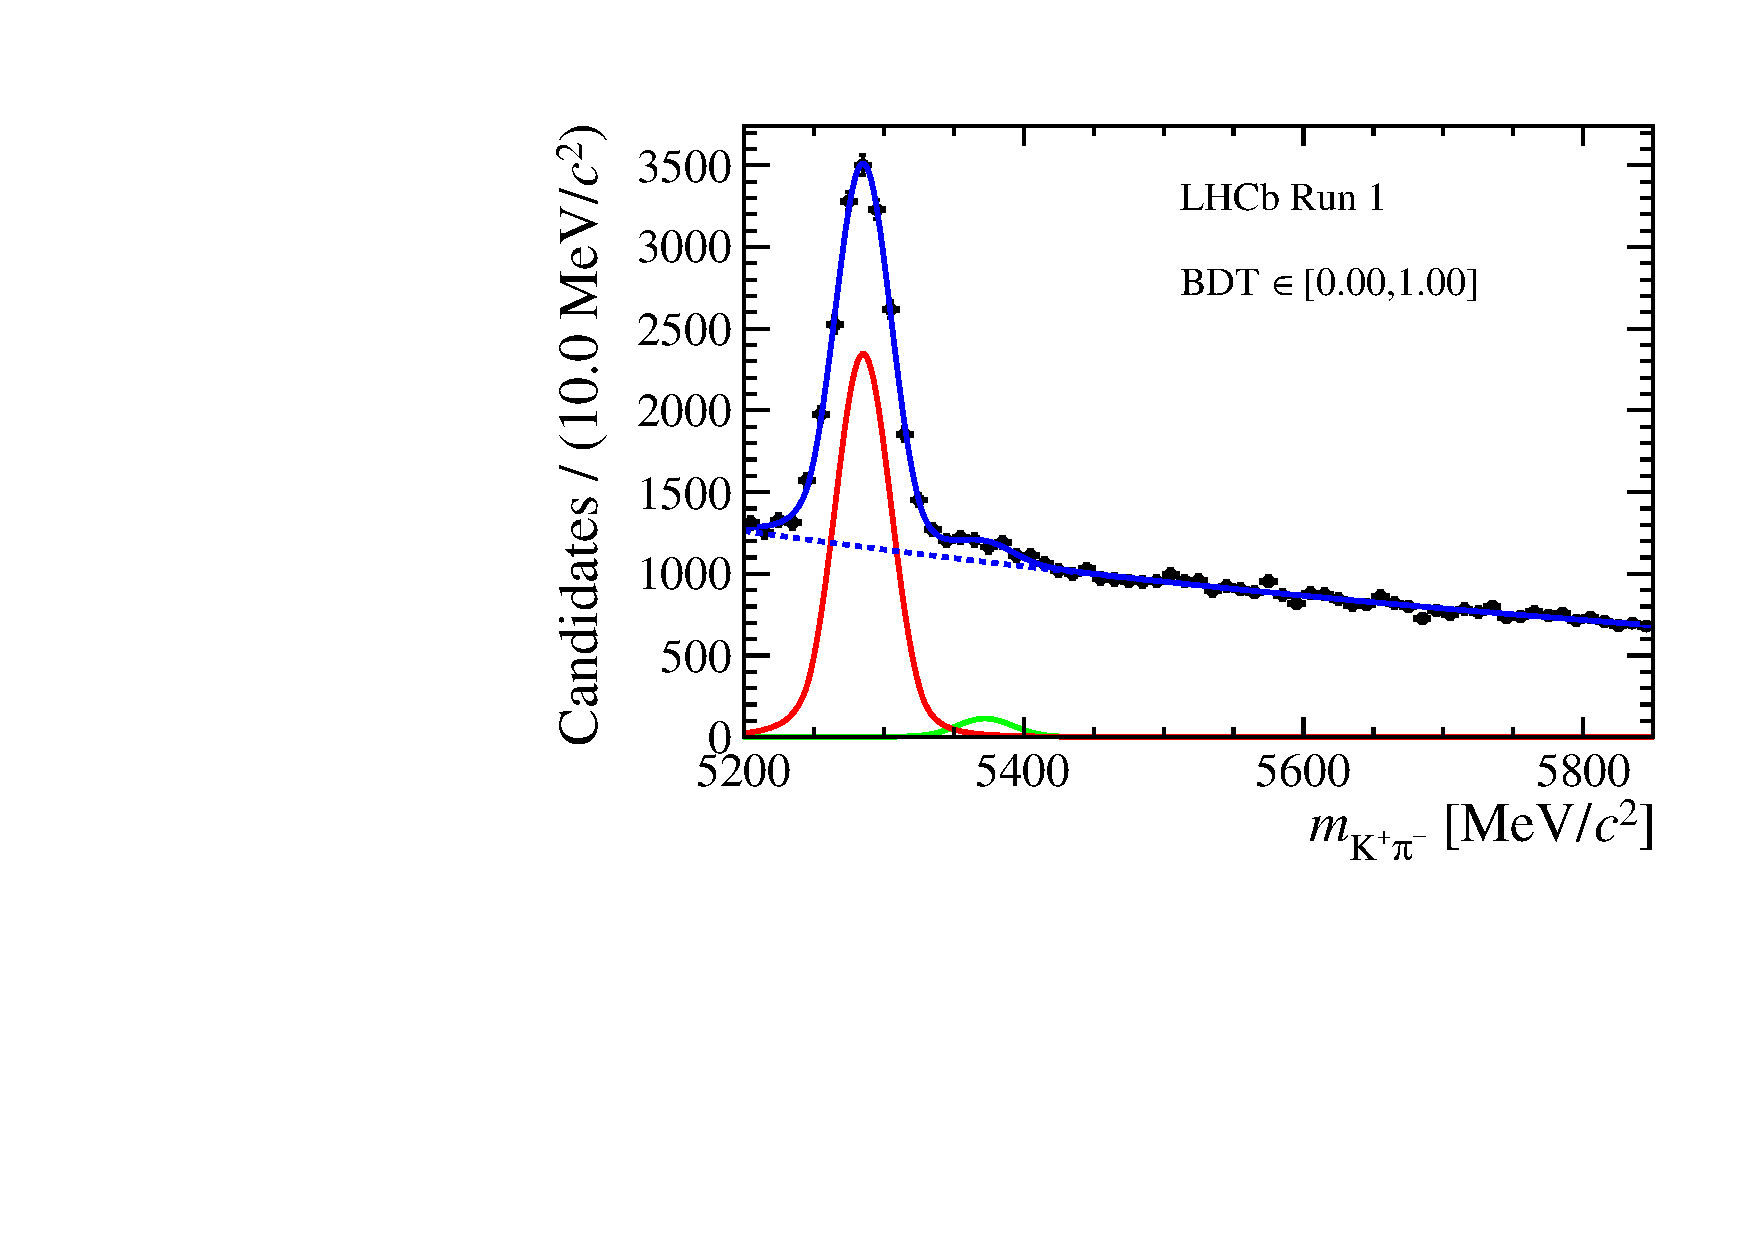
\includegraphics[width=  \textwidth]{./Figs/BFAnalysis/Bd2KPi_mass_RunI_BDTbinNone.pdf}
        %\caption{ }
       % \label{fig:BDTSsig}
    \end{subfigure}
   % ~ %add desired spacing between images, e. g. ~, \quad, \qquad, \hfill etc. 
      %(or a blank line to force the subfigure onto a new line)
    \begin{subfigure}[b]{0.4\textwidth}
       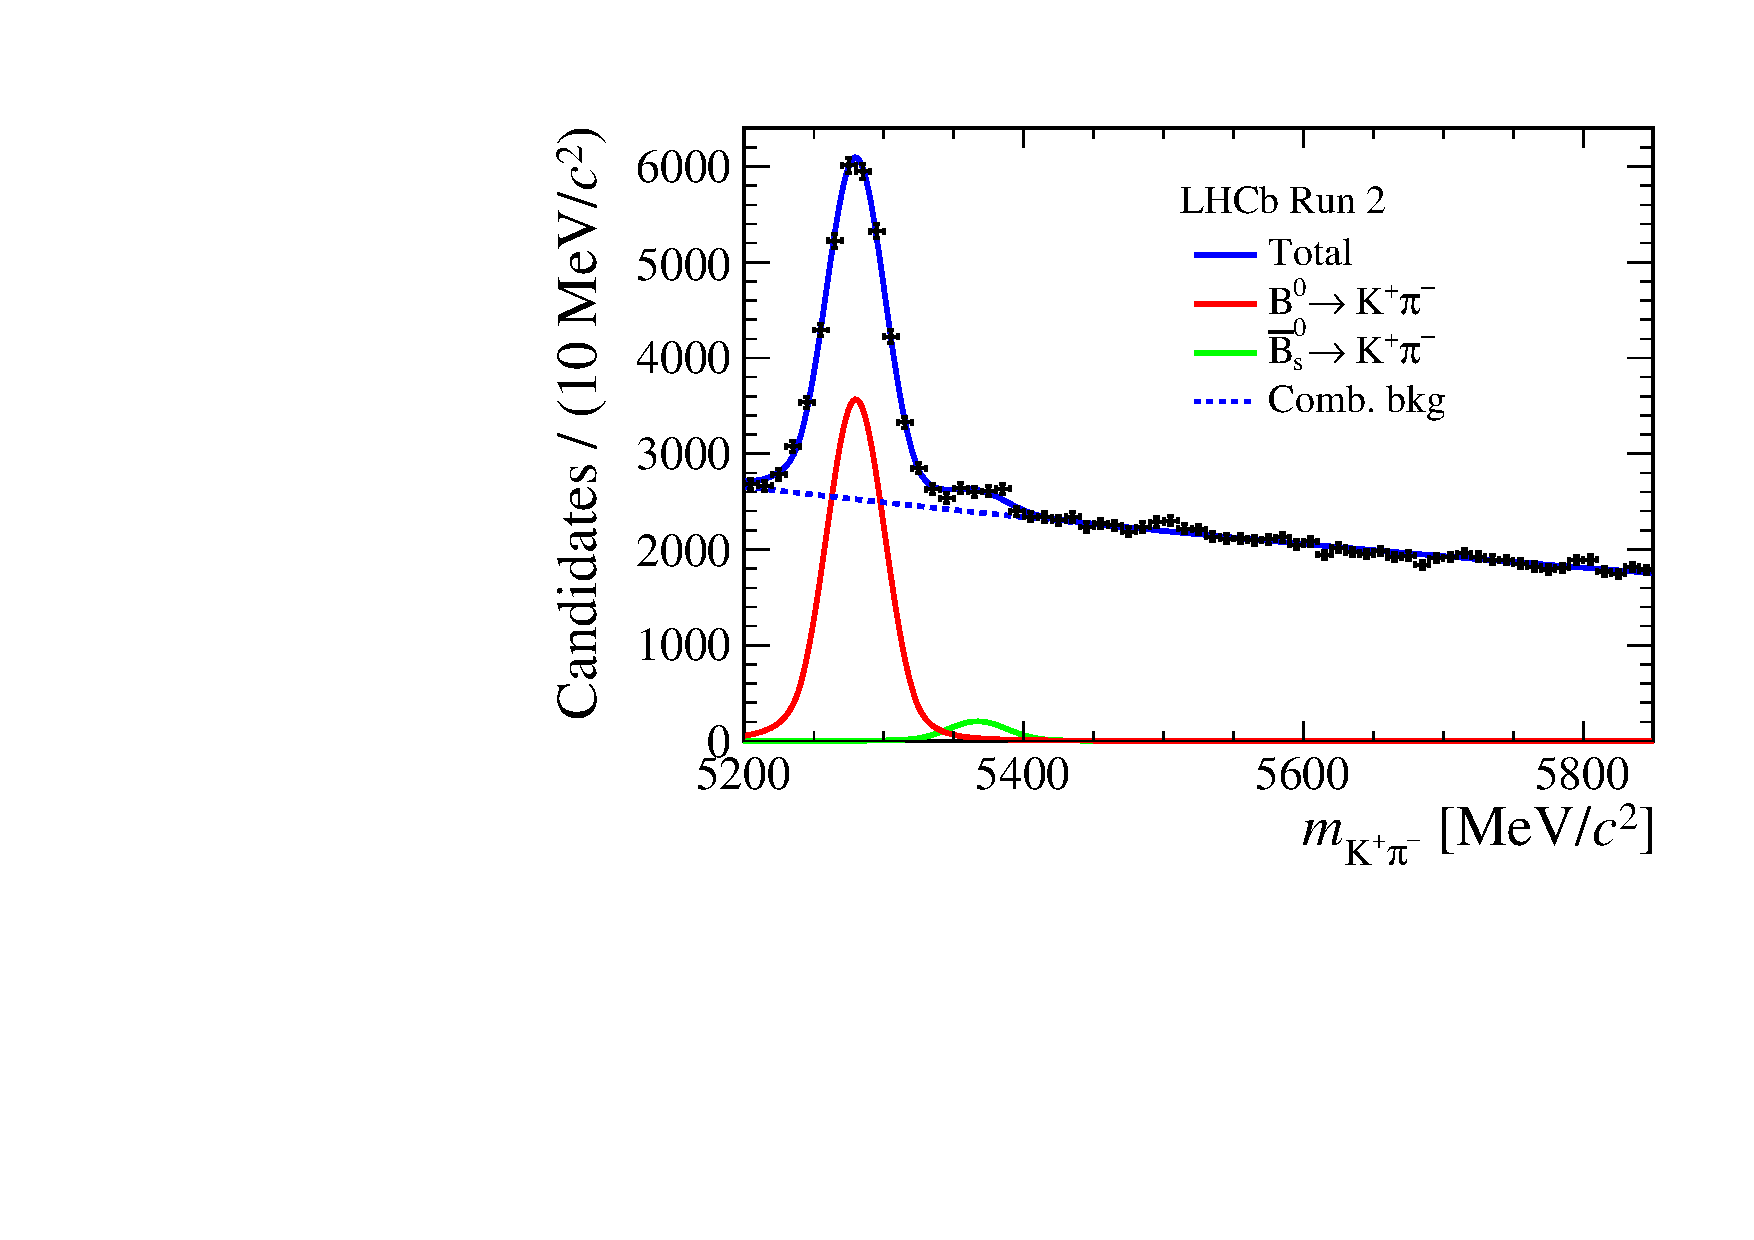
\includegraphics[width=\textwidth]{./Figs/BFAnalysis/Bd2KPi_mass_RunII_BDTbinNone.pdf}
      %  \caption{ }
     %   \label{fig:BDTSbkg}
   \end{subfigure}
    \caption{Mass fit to measure \bdkpi yield for the noramlisation for Run 1 (left) and Run 2 (right) data. }
    \label{fig:Bdkpiyield}
\end{figure}



\begin{figure}[htbp]
    \centering
   \begin{subfigure}[b]{0.4\textwidth}
        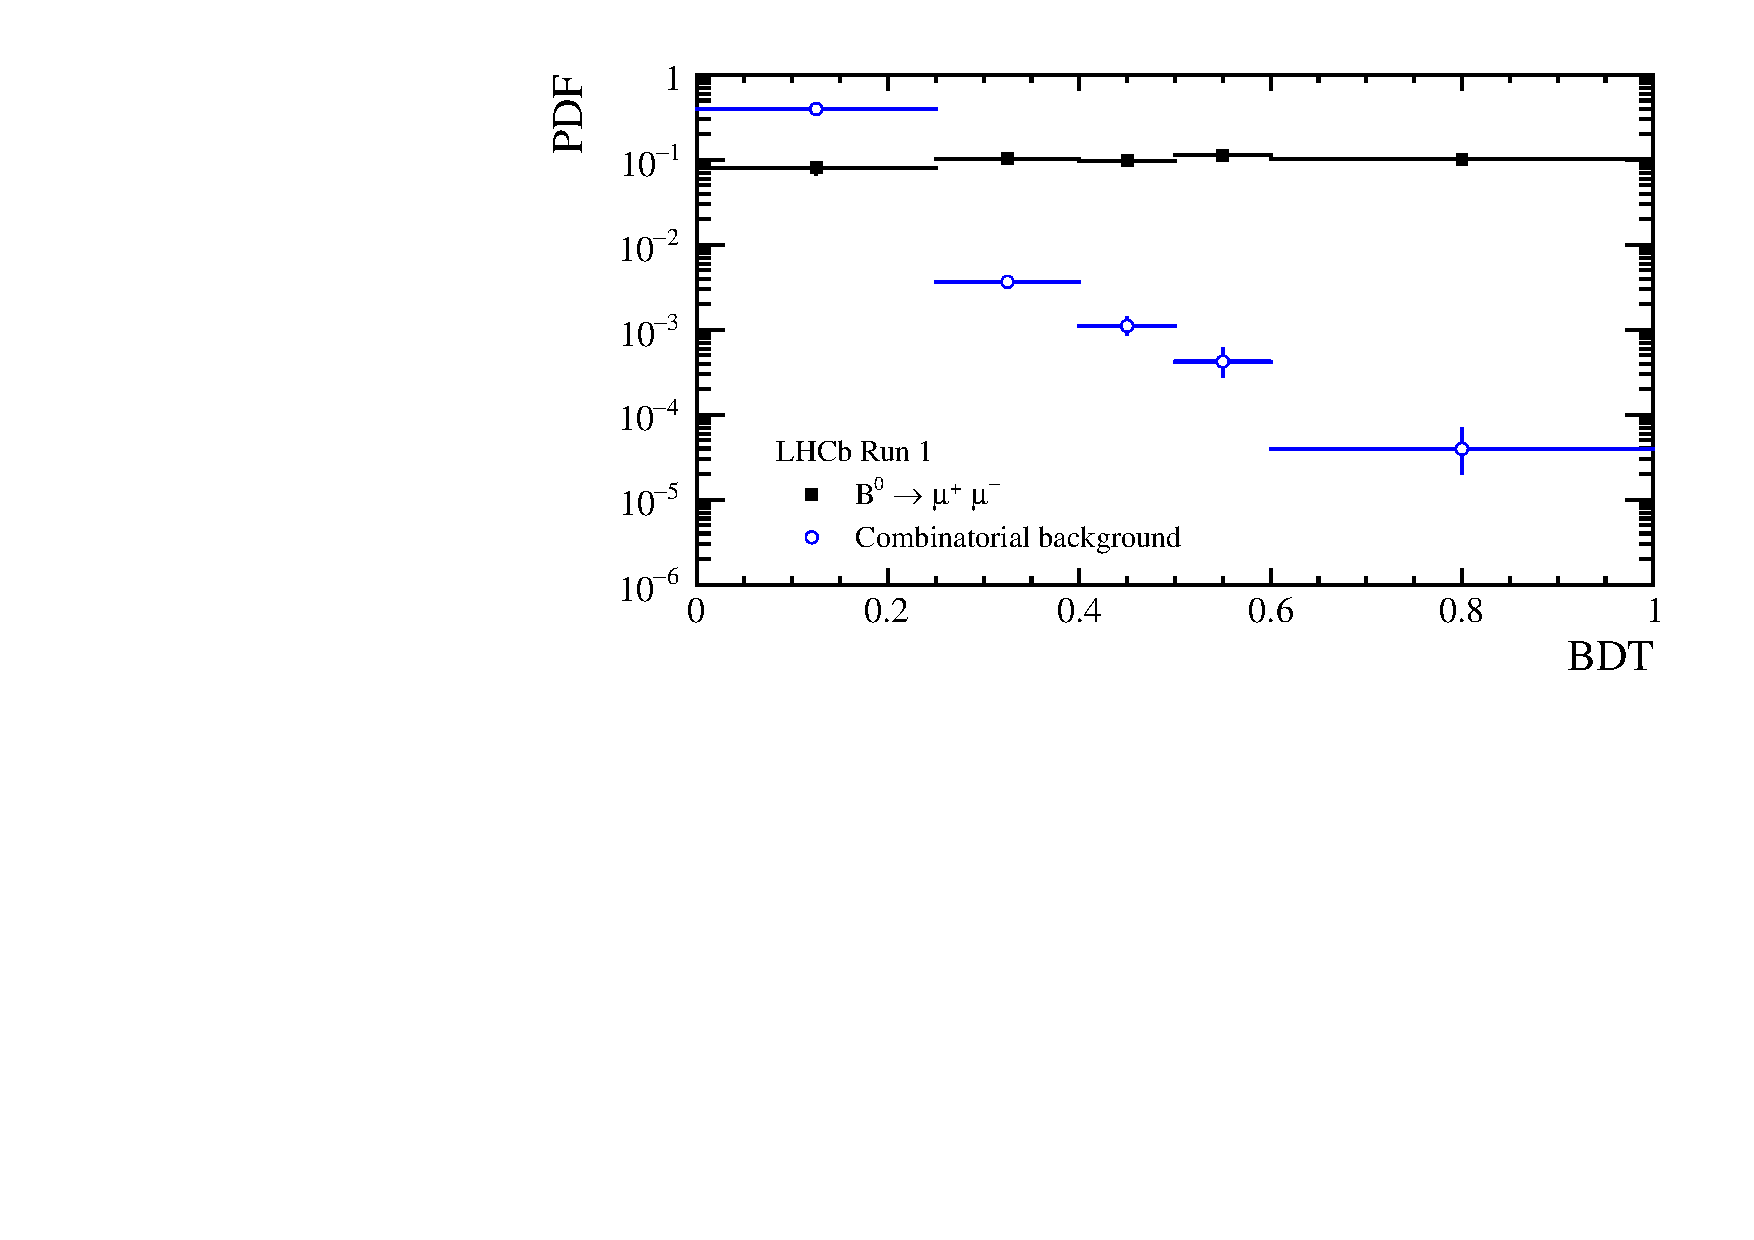
\includegraphics[width=  \textwidth]{./Figs/BFAnalysis/Bd2KPi_BDTCalibration_RunI.pdf}
        %\caption{ }
       % \label{fig:BDTSsig}
    \end{subfigure}
   % ~ %add desired spacing between images, e. g. ~, \quad, \qquad, \hfill etc. 
      %(or a blank line to force the subfigure onto a new line)
    \begin{subfigure}[b]{0.4\textwidth}
       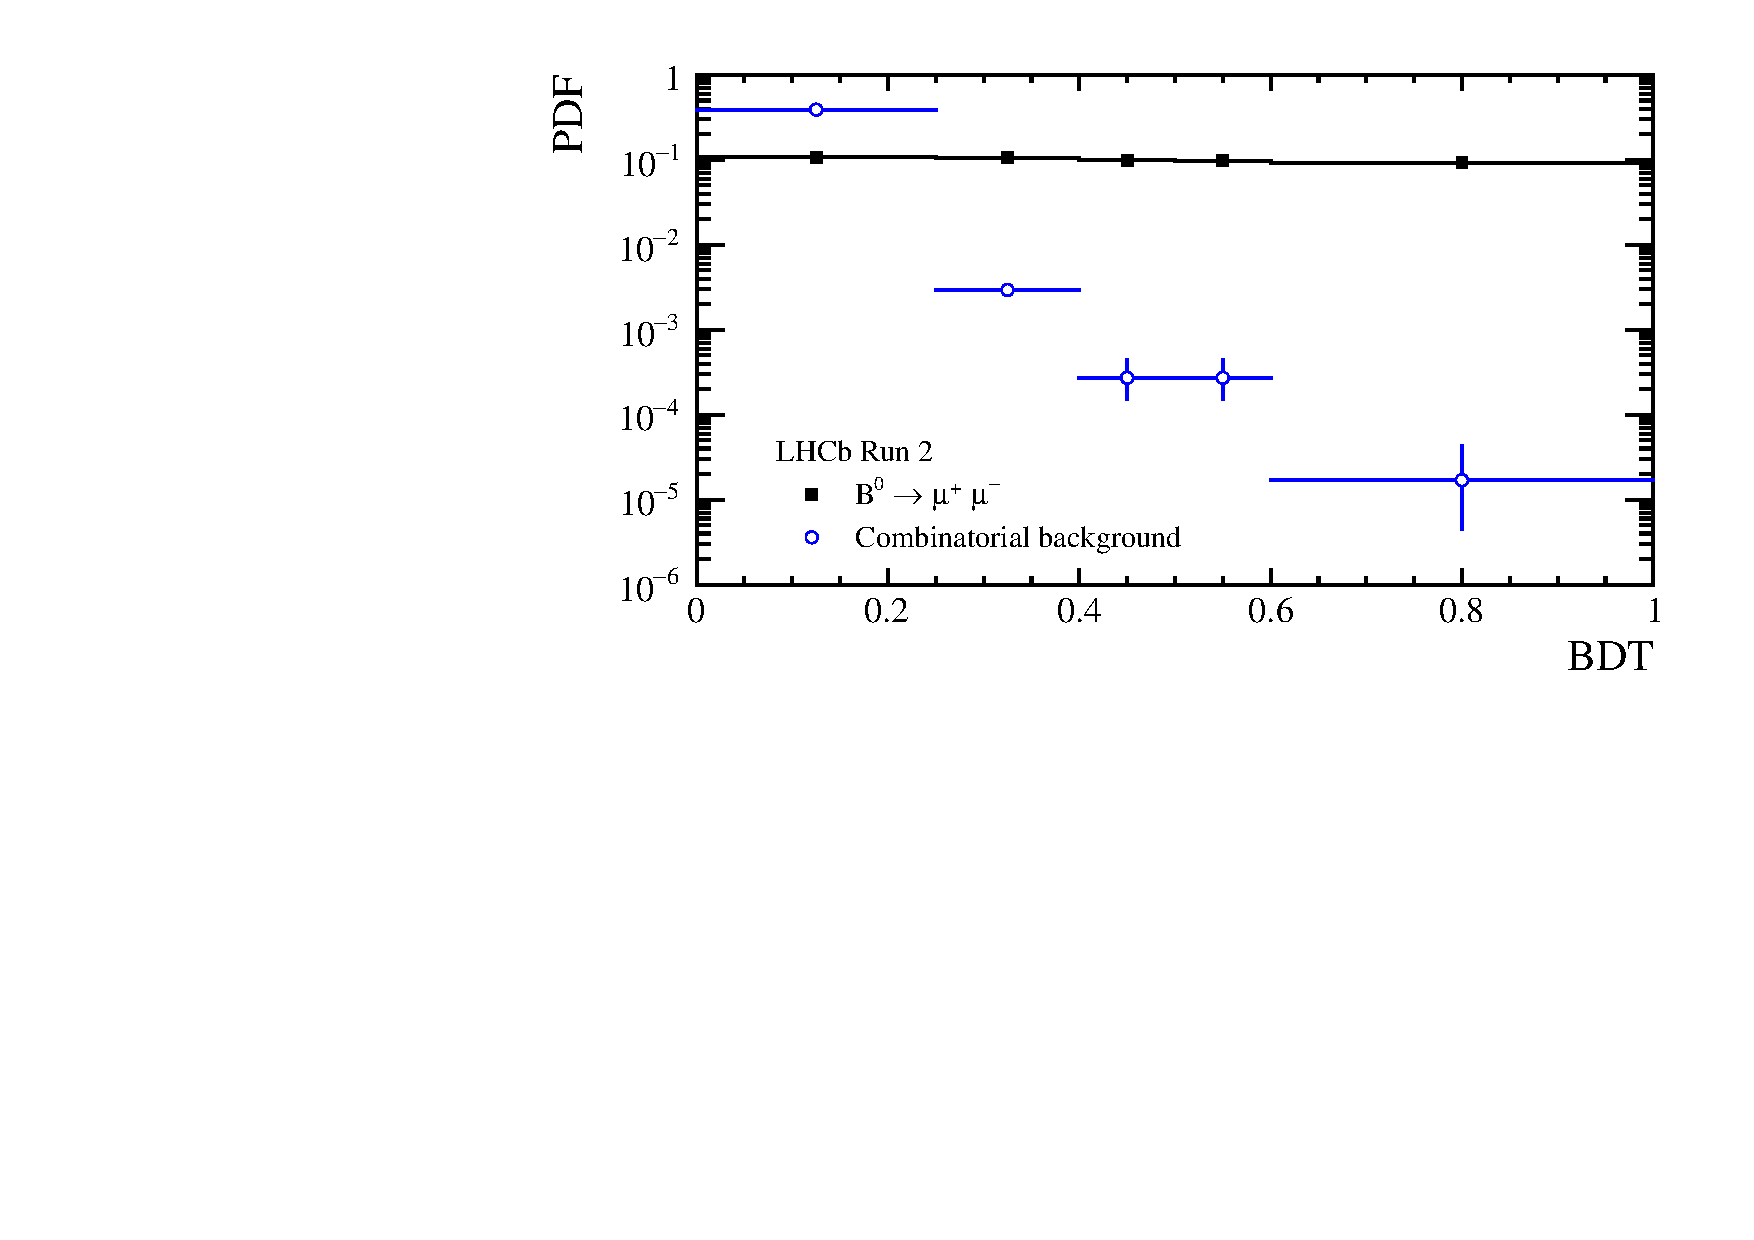
\includegraphics[width=\textwidth]{./Figs/BFAnalysis/Bd2KPi_BDTCalibration_RunII.pdf}
      %  \caption{ }
     %   \label{fig:BDTSbkg}
   \end{subfigure}
    \caption{ Mass fit to measure \bujpsik yield for the noramlisation for Run 1 (left) and Run 2 (right) data.}
    \label{fig:Bujpsikyield}
\end{figure}


\subsection{Efficiencies}
The normalisation factors require various efficienciey for identifying \bmumu, \bdkpi and \bujpsik decays to be evalutated for each year of data taking. % and using the full BDT range. %The efficiencies in equation X are defined as:

The acceptance efficiency, , gives the efficiency for the decay products to be within the LHCb detector acceptance. This efficiency is evaluated on simulated decays to for decay products that fall within the range [10,400] mrad. The range is chosen to be slighly larger than the detector acceptance so that particles recoved by the magnetic field are included. To keep this efficienciy similar for \bmumu and \bdkpi decays, the hadrons from \bdkpi are required to be within the muon detector acceptance. 

The reconstruction efficiencu of decays that are within the detector acceptance and the selection efficiency of reconstructed decays is given by . The selection and reconstruction efficiencies are evaluated from a combination of information from data and simulated decays to ensure accurate selection efficiency ratios. Similar to the BDT PDF a correction is applied for the lifetime used in simulated \bsmumu decays assuming \ADG = +1. 

The trigger efficiencies for decays passing the reconstruction and selection, , are evalutaed by data driven methods as descrided in~\ref{}. 

The efficiencies are caluculated for \bsmumu, \bdmumu, \bdkpi and \bujpsik seperatly to account for difference in the decays and kinematics.

\subsection{Hadronisation factors}

The normalisation factors depend on hadronisation factors, $f_{u}, f_{s}, f_{d}$, that give the probability of a $b$ or $\bar{b}$ quark to form a particular $B^{+}$, \bs or \bd, respectively. The hadronisation factors $f_{d}$ and $f_{u}$ are equal therefore the \bmumu bracnhing fraction does not depend on any hadronisation factors. For the \bsmumu the ratio $f_{s}/f_{d}$ is used in the noramlisation, since $f_{d} = f_{u}$. This ratio was measured at LHCb for $pp$ collisions at $\sqrt{s}$ = 7 TeV, and a comparison of the number of \bujpsik and \bsjpisphi decays shows it is consistent across the different LHC energies. However for Run 2 the $f_{s}/f_{d}$ ratio must be modified for the small observed realtive production difference. {\it Is this too much detail?}
The unceratinty on the hadronisation factor ratio contributes the larges unceratiny to the \bsmumu branching fraction. Alternatively the \bsmumu decay could be noramlisated using a different \bs decay however the precision of the measured branching fractions and adundance of \bs decays, such as \bsjpsiphi, are not high enough at present to provide a lower overall uncertainty on the noramalisation factors than the $f_{s}/f_{d}$ ratio.


The various yields, efficiencies and hadronisation factors are combined to produce seperate normalisation factors for each year of data taking and each noramlisation channel. The factors are combined to produced one set of normalisation factors for Run 1 and for Run 2.  {\it I could put the yearly equation in and say that the weighted average is taken of the two modes?}. The \bujpsik noramlisation factors are also used in determining the number of expected background decays in each BDT bin as detail in the earlier Section X. 


\section{Results}

As described in Section X the \bsmumu and \bmumu branching fractions are measured by a simulatanous maximum likelihood fit to the dimuon invariant mass of the Run 1 and Run 2 data sets, each divided into four BDT bins. 

In the fit the mass pdfs and fraction of \bmumu decays in each BDT bin are constained within Gaussain limits using their expected values and unceratinties. The yield of the combinatorial background is left free in the fit in each BDT bin and the slope of the mass distribution is constained to have the same value accross all bins for each data set. The backgrounds from \bhh, \bdpimunu, \bsKmunu, \bpimumu, \bdpimumu and \bcjpsimunu decays have their yields and fractions in each BDT bin constrained around the expected values, similarly to the signal fractions but the mass shapes are fixed in the fit.

The branching fraction results from the fit are;

\begin{eqnarray}
%\begin{align}
  \mathcal{B}(B^{0}_{s} \to \mu^{+} \mu^{-}) &=& (2.8 \pm 0.6) \times 10^{-9} \\
  \mathcal{B}(B^{0} \to \mu^{+} \mu^{-}) &=& (1.6^{+1.1}_{-0.9})    \times 10^{-10} 
%\end{align}
\label{eq:BFresults}
\end{eqnarray}
Figure~\ref{fig:MLfit} shows the fit results for \bmumu candidates with a global BDT $> 0.5$ and Figure~\ref{fig:contour} the 2-dimensioanly likelihood profile for the \bdmumu and \bsmumu branching fraction measurements.
The statistics significancal of the \bsmumu signal is 7.9 $\sigma$ which is the first single experiment obseravtion of the \bsmumu decay. While the significance of the \bdmumu signal is less at 1.9$\sigma$, therefore the CLs method is used to place an upper limit on the branching fraction of $\mathcal{B}(\bdmumu) < 3.4 \times 10^{-10}$  at the 95 $\%$ confidence level.

The quoted \bsmumu branching fraction assumes the SM value for \ADG, applying the corrections detailed in Section X for \ADG values of 0 and -1 shift the central value of $\mathcal{B}(\bsmumu)$ by 4.6 $\%$ and 10.9 $\%$, respectively. 


{\it  This could either go in this section or the overview - I'm not sure which is best since it references stuff so may be better here but sounds a bit odd ... ??}






\begin{figure}[htbp]
    \centering
        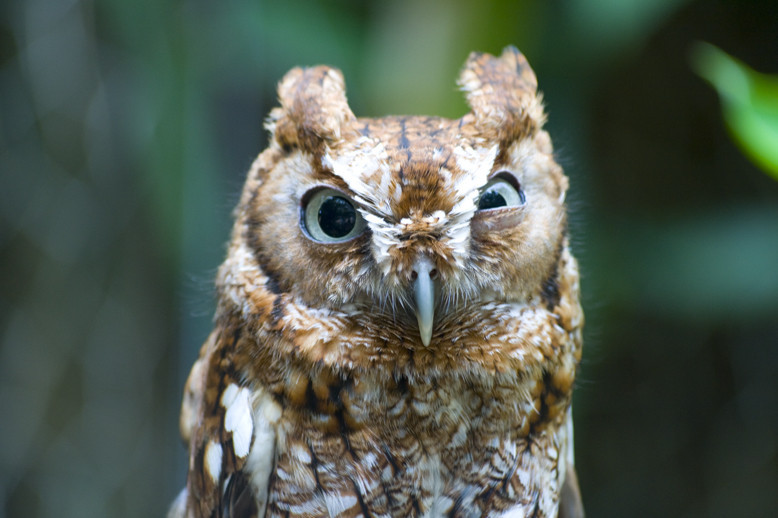
\includegraphics[width= 0.8 \textwidth]{./Figs/BFAnalysis/placeholder.jpeg}
      \caption{2D likelihood for \bd and \bs BFs. }
    \label{fig:contour}
\end{figure}


\begin{figure}[htbp]
    \centering
    \begin{subfigure}[b]{0.48\textwidth}
        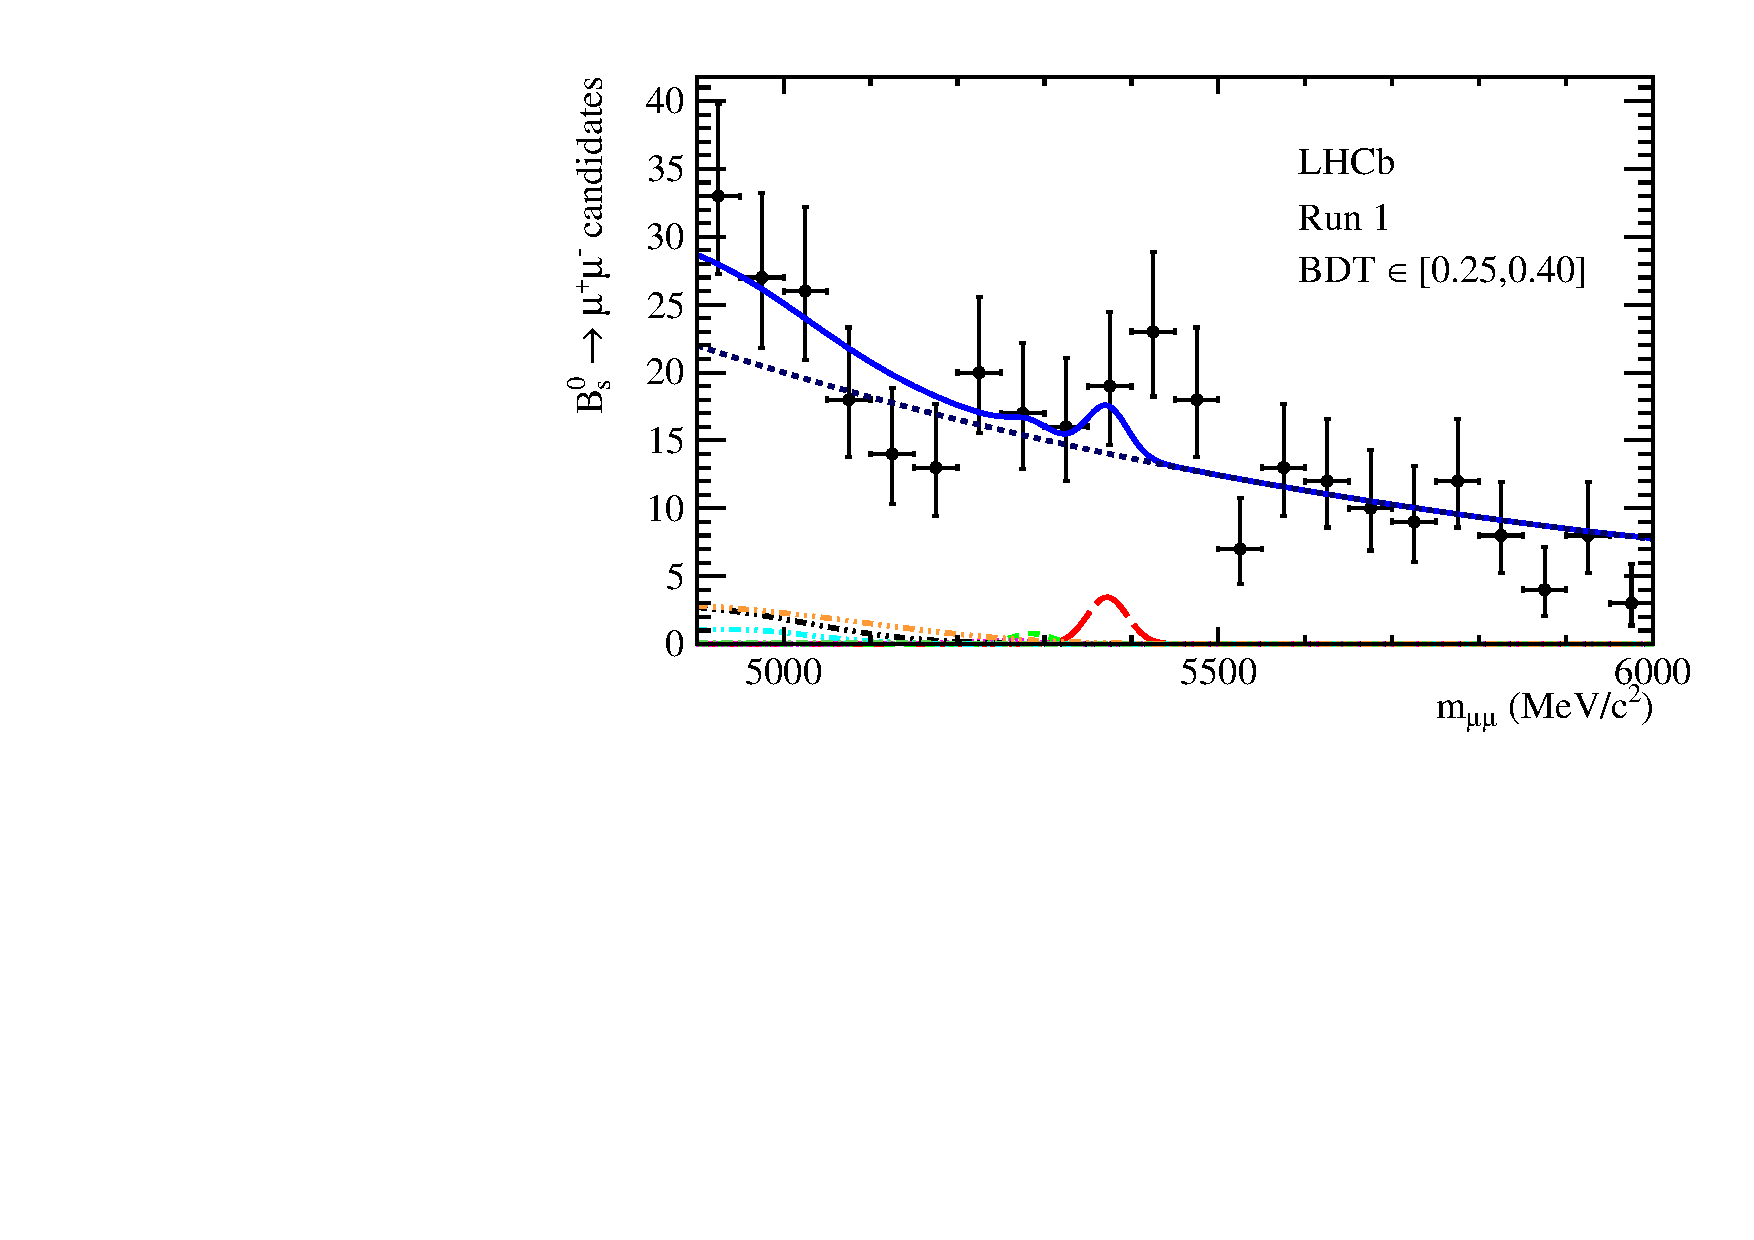
\includegraphics[width=\textwidth]{./Figs/BFAnalysis/Bsmumu_Fit_Run1_bin2.pdf}
    \end{subfigure}
    ~ %add desired spacing between images, e. g. ~, \quad, \qquad, \hfill etc. 
      %(or a blank line to force the subfigure onto a new line)
    \begin{subfigure}[b]{0.48\textwidth}
       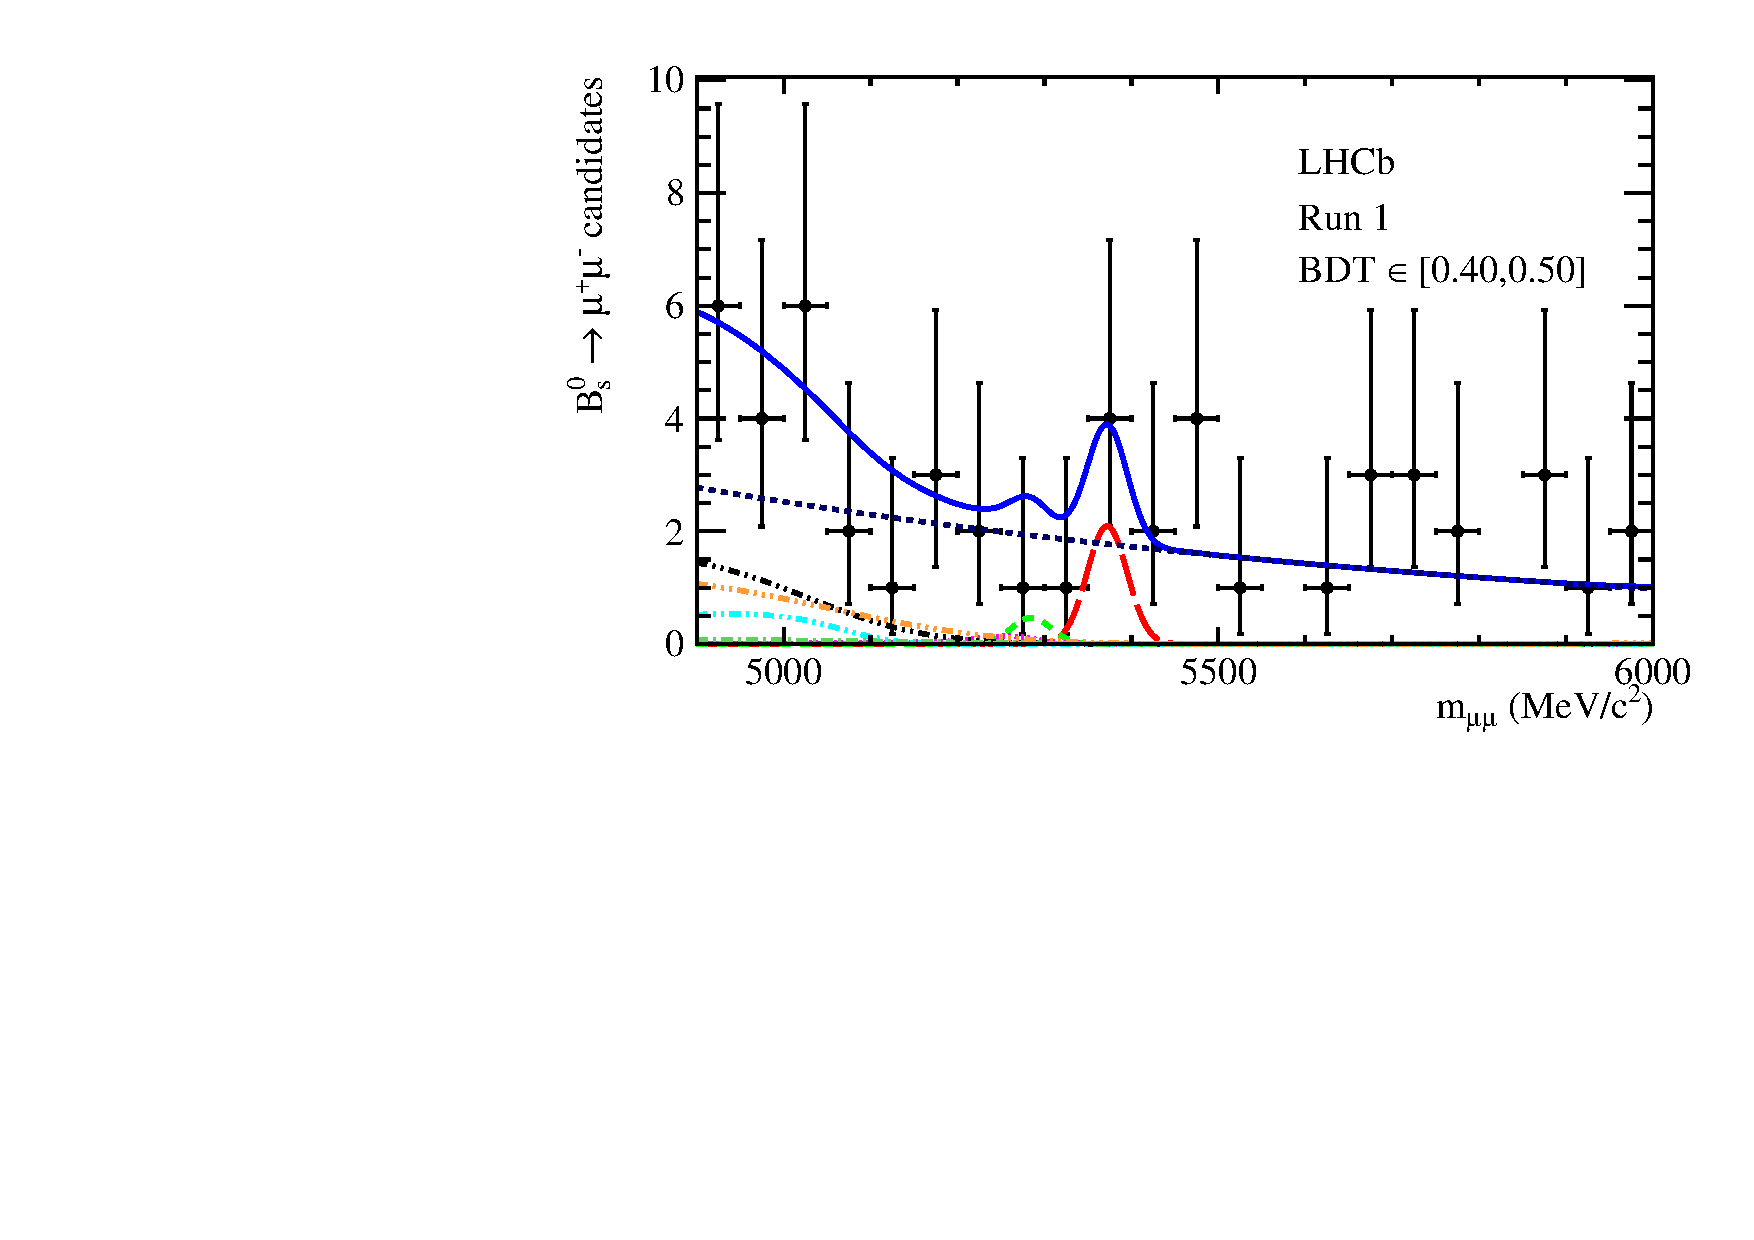
\includegraphics[width=\textwidth]{./Figs/BFAnalysis/Bsmumu_Fit_Run1_bin3.pdf}
    \end{subfigure}
    \begin{subfigure}[b]{0.48\textwidth}
        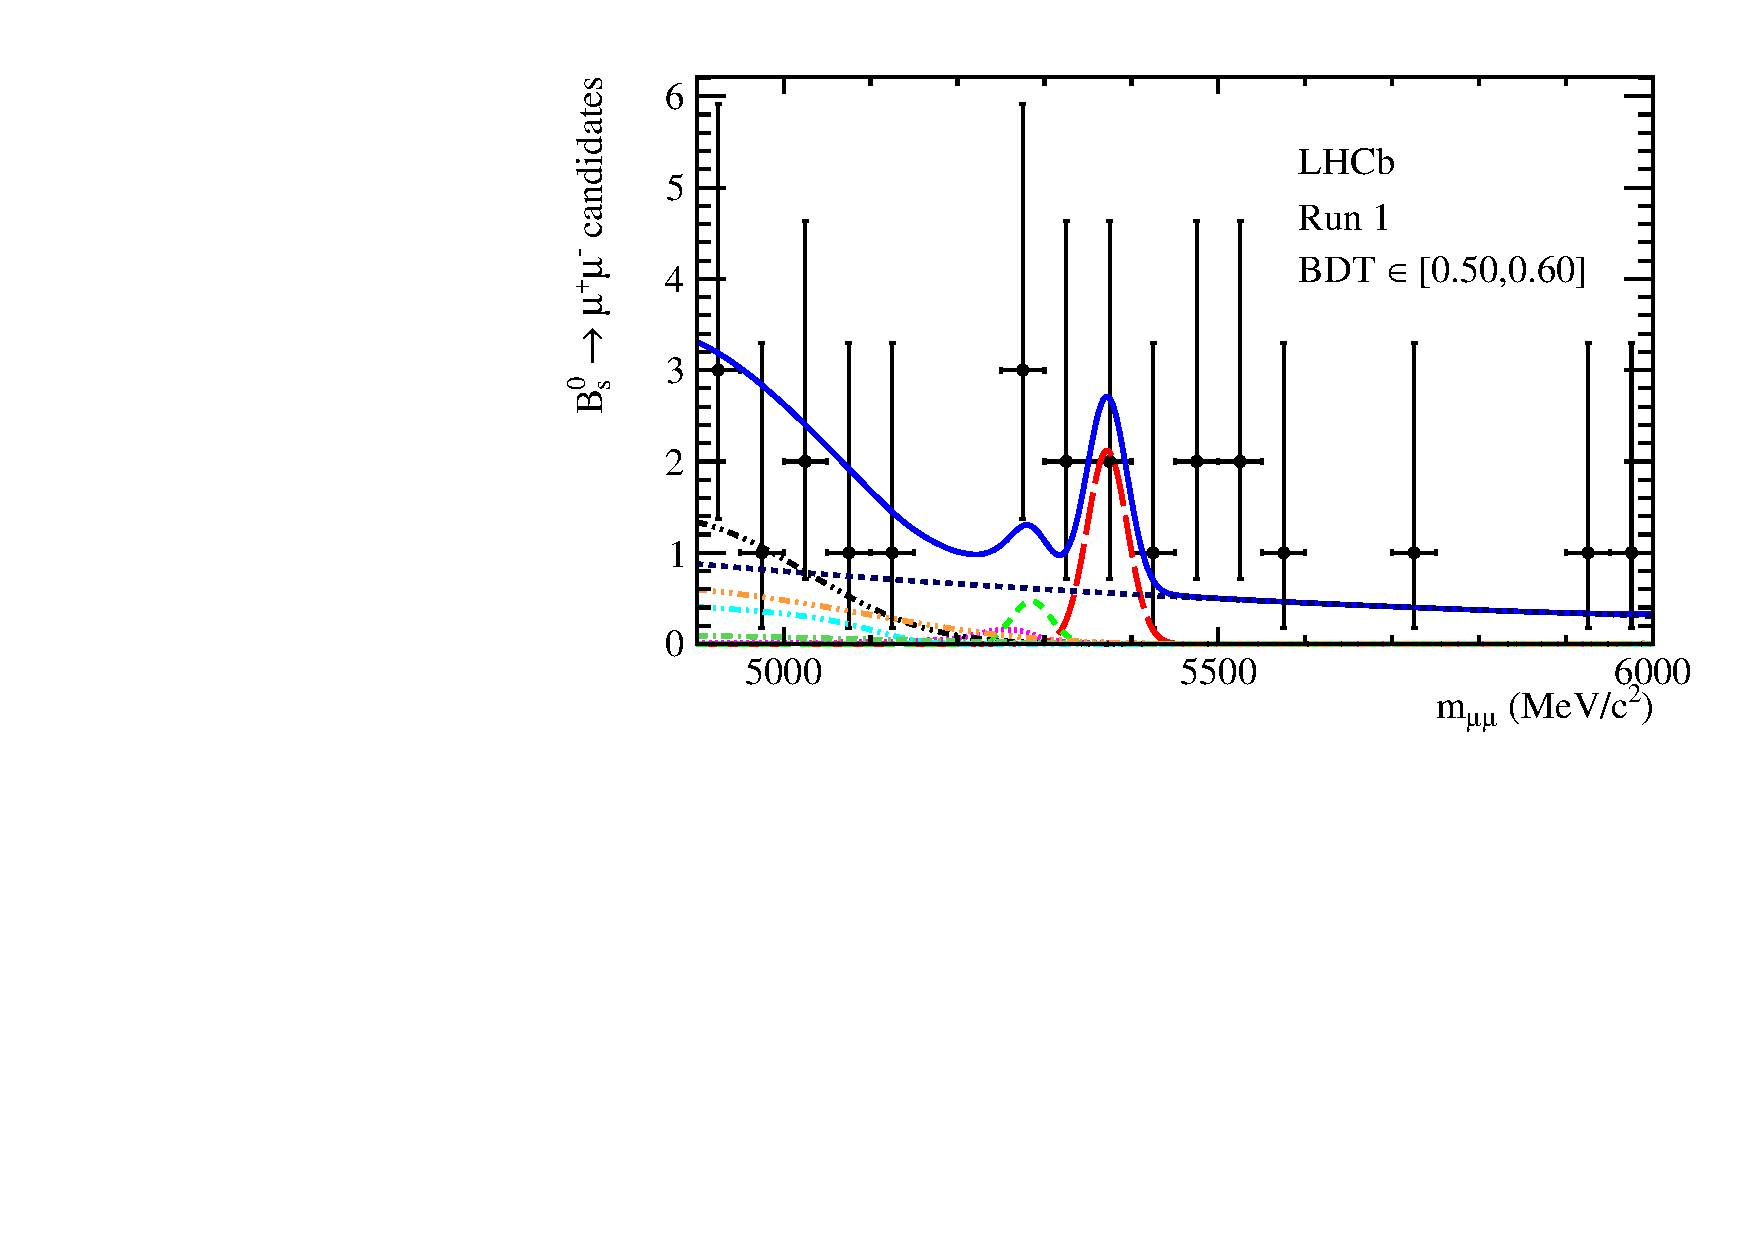
\includegraphics[width=\textwidth]{./Figs/BFAnalysis/Bsmumu_Fit_Run1_bin4.pdf}
    \end{subfigure}
    ~ %add desired spacing between images, e. g. ~, \quad, \qquad, \hfill etc. 
      %(or a blank line to force the subfigure onto a new line)
    \begin{subfigure}[b]{0.48\textwidth}
       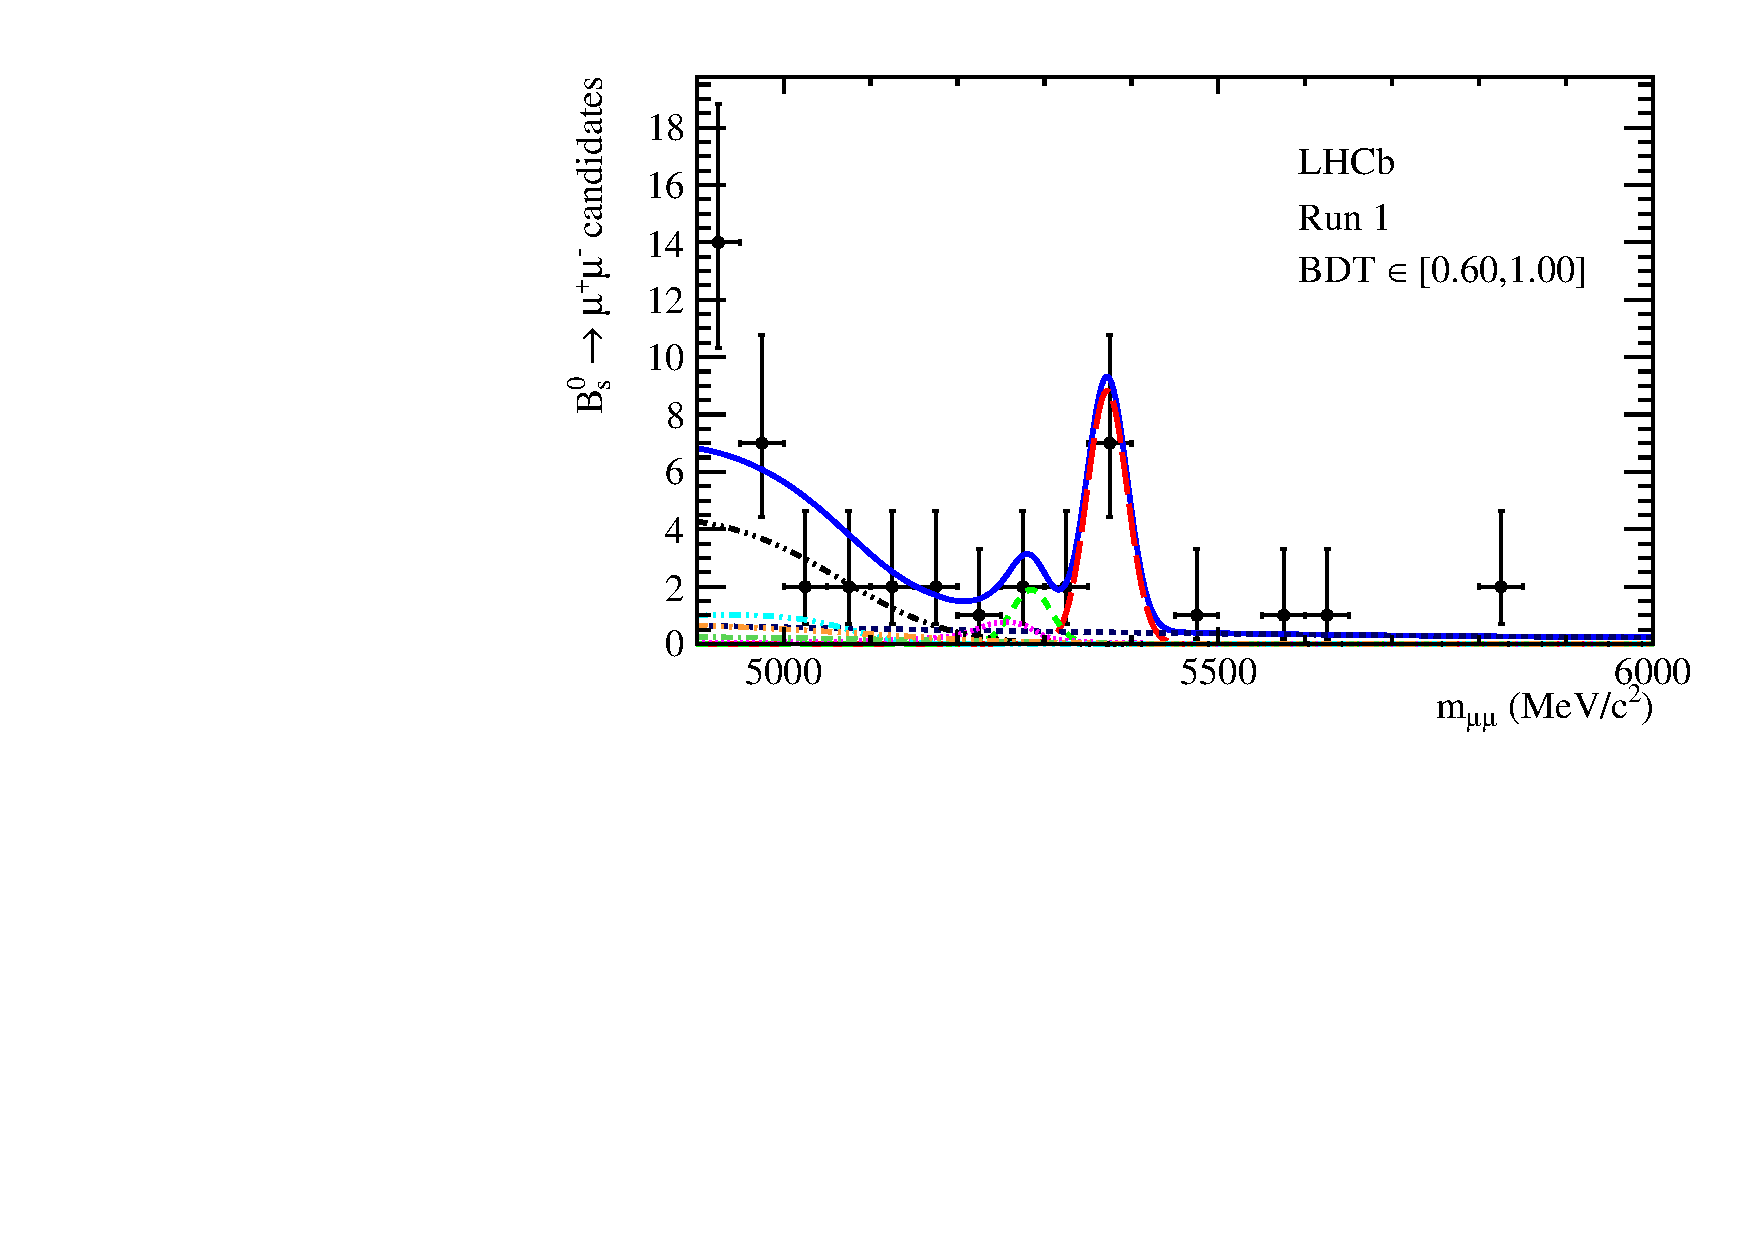
\includegraphics[width=\textwidth]{./Figs/BFAnalysis/Bsmumu_Fit_Run1_bin5.pdf}
    \end{subfigure}

    \qquad

    \begin{subfigure}[b]{0.48\textwidth}
        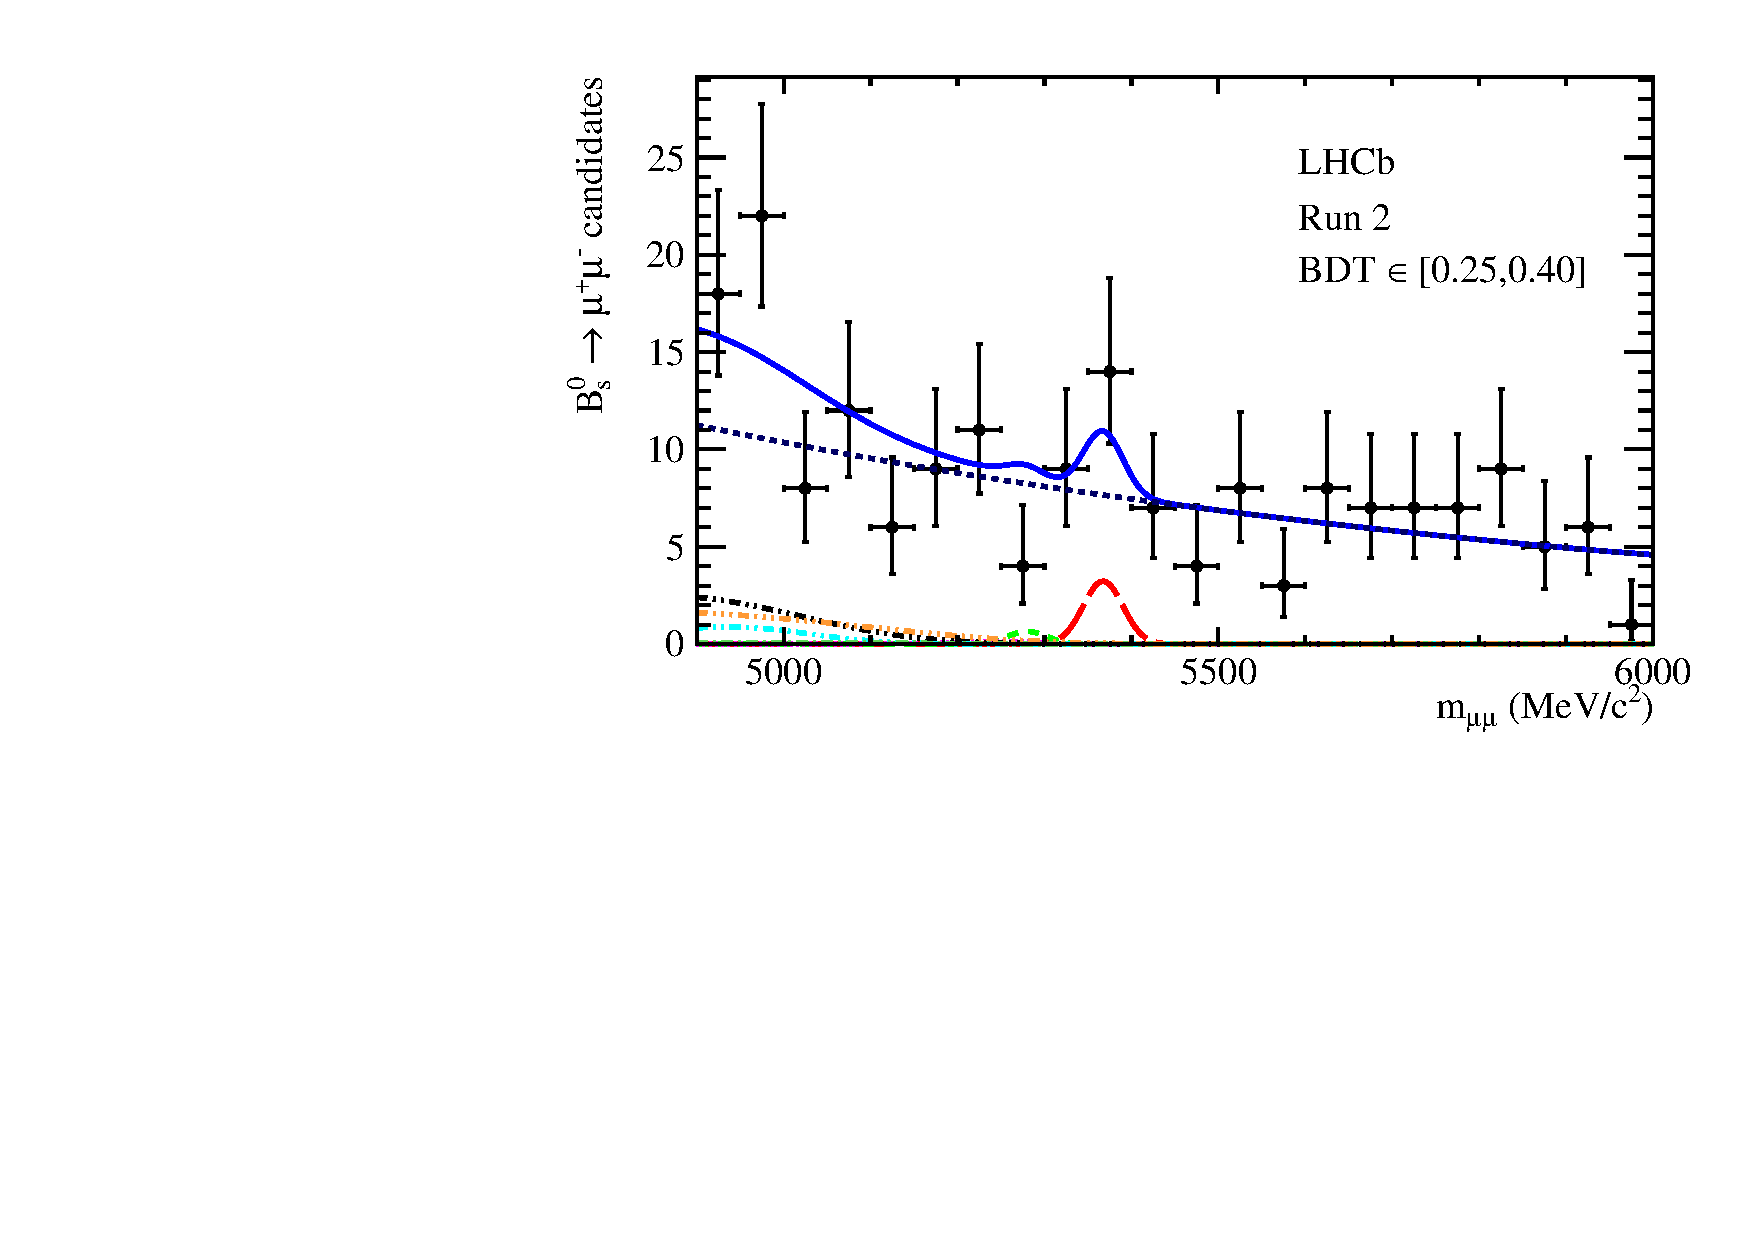
\includegraphics[width=\textwidth]{./Figs/BFAnalysis/Bsmumu_Fit_Run2_bin2.pdf}
    \end{subfigure}
    ~ %add desired spacing between images, e. g. ~, \quad, \qquad, \hfill etc. 
      %(or a blank line to force the subfigure onto a new line)
    \begin{subfigure}[b]{0.48\textwidth}
       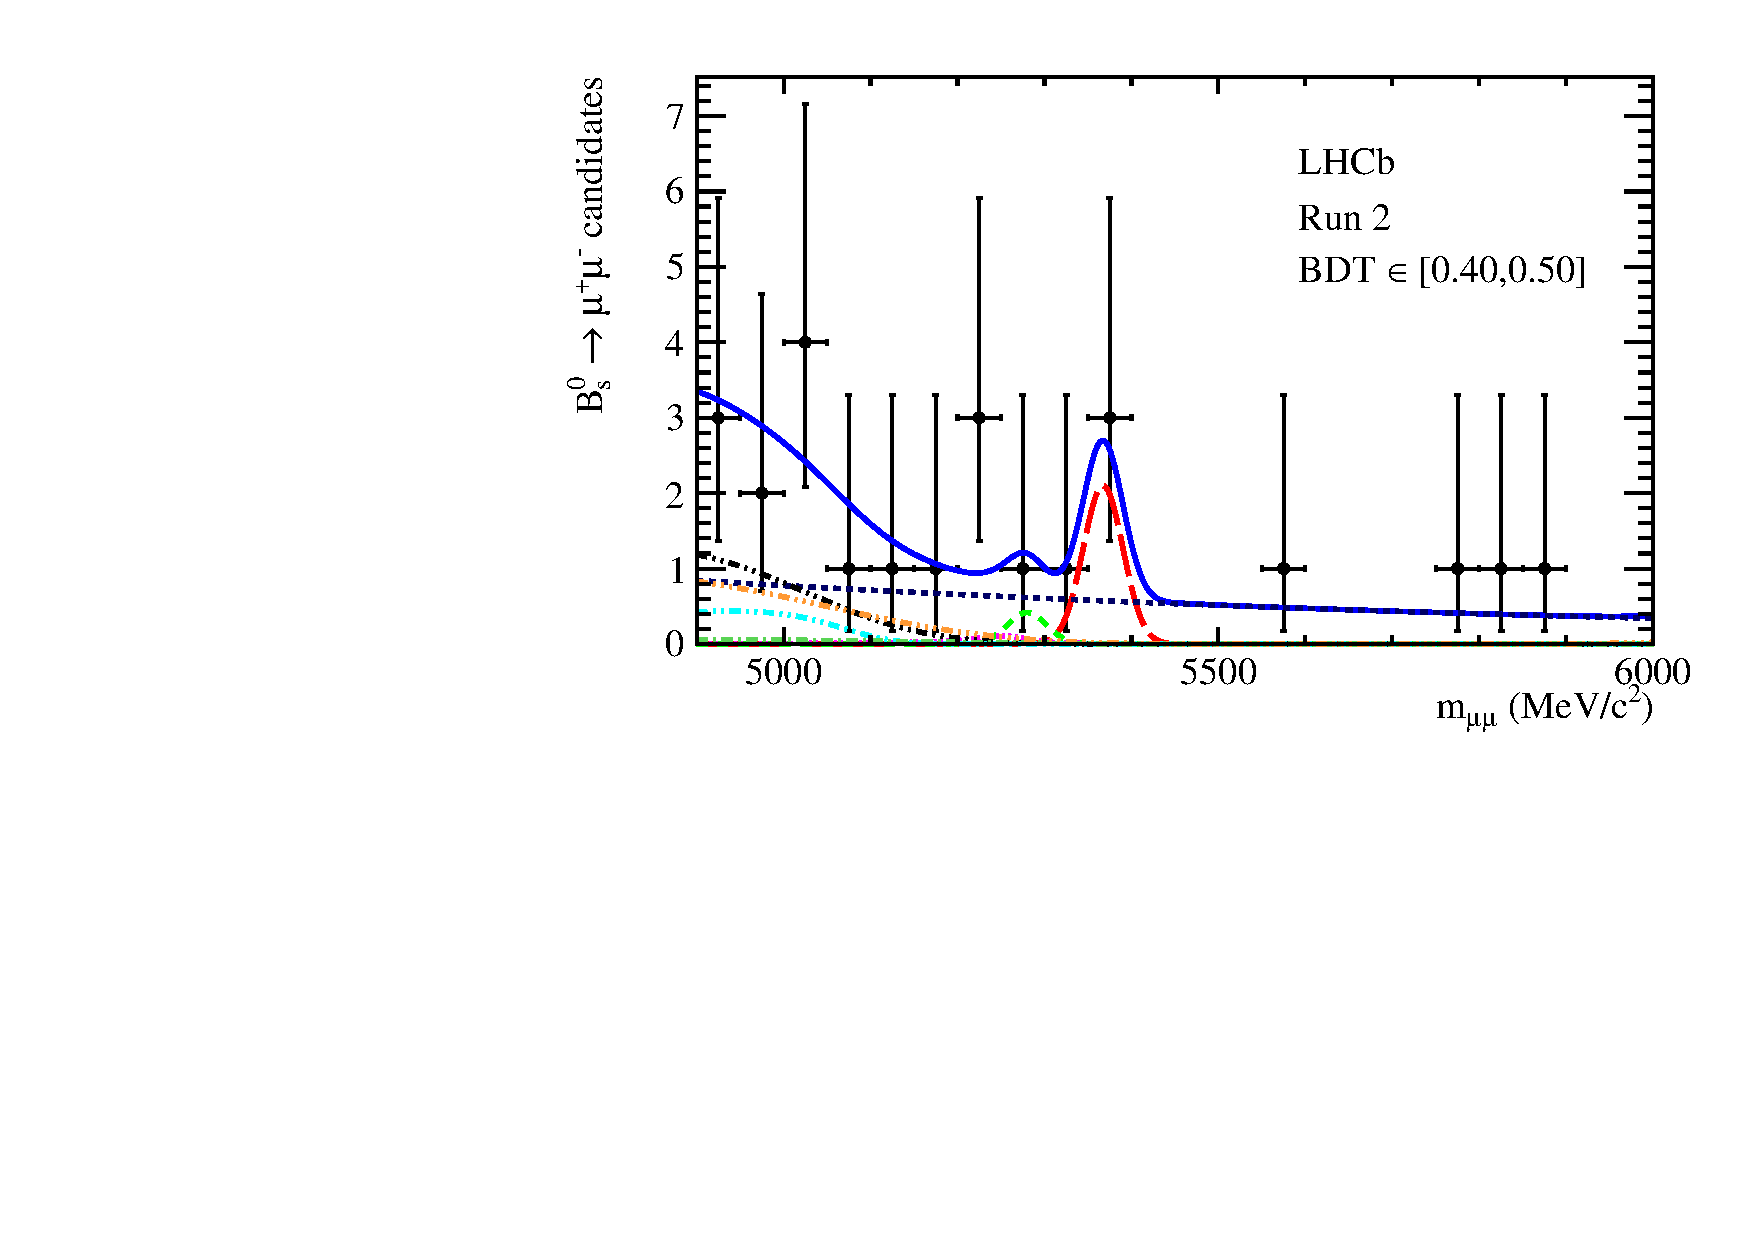
\includegraphics[width=\textwidth]{./Figs/BFAnalysis/Bsmumu_Fit_Run2_bin3.pdf}
    \end{subfigure}
    \begin{subfigure}[b]{0.48\textwidth}
        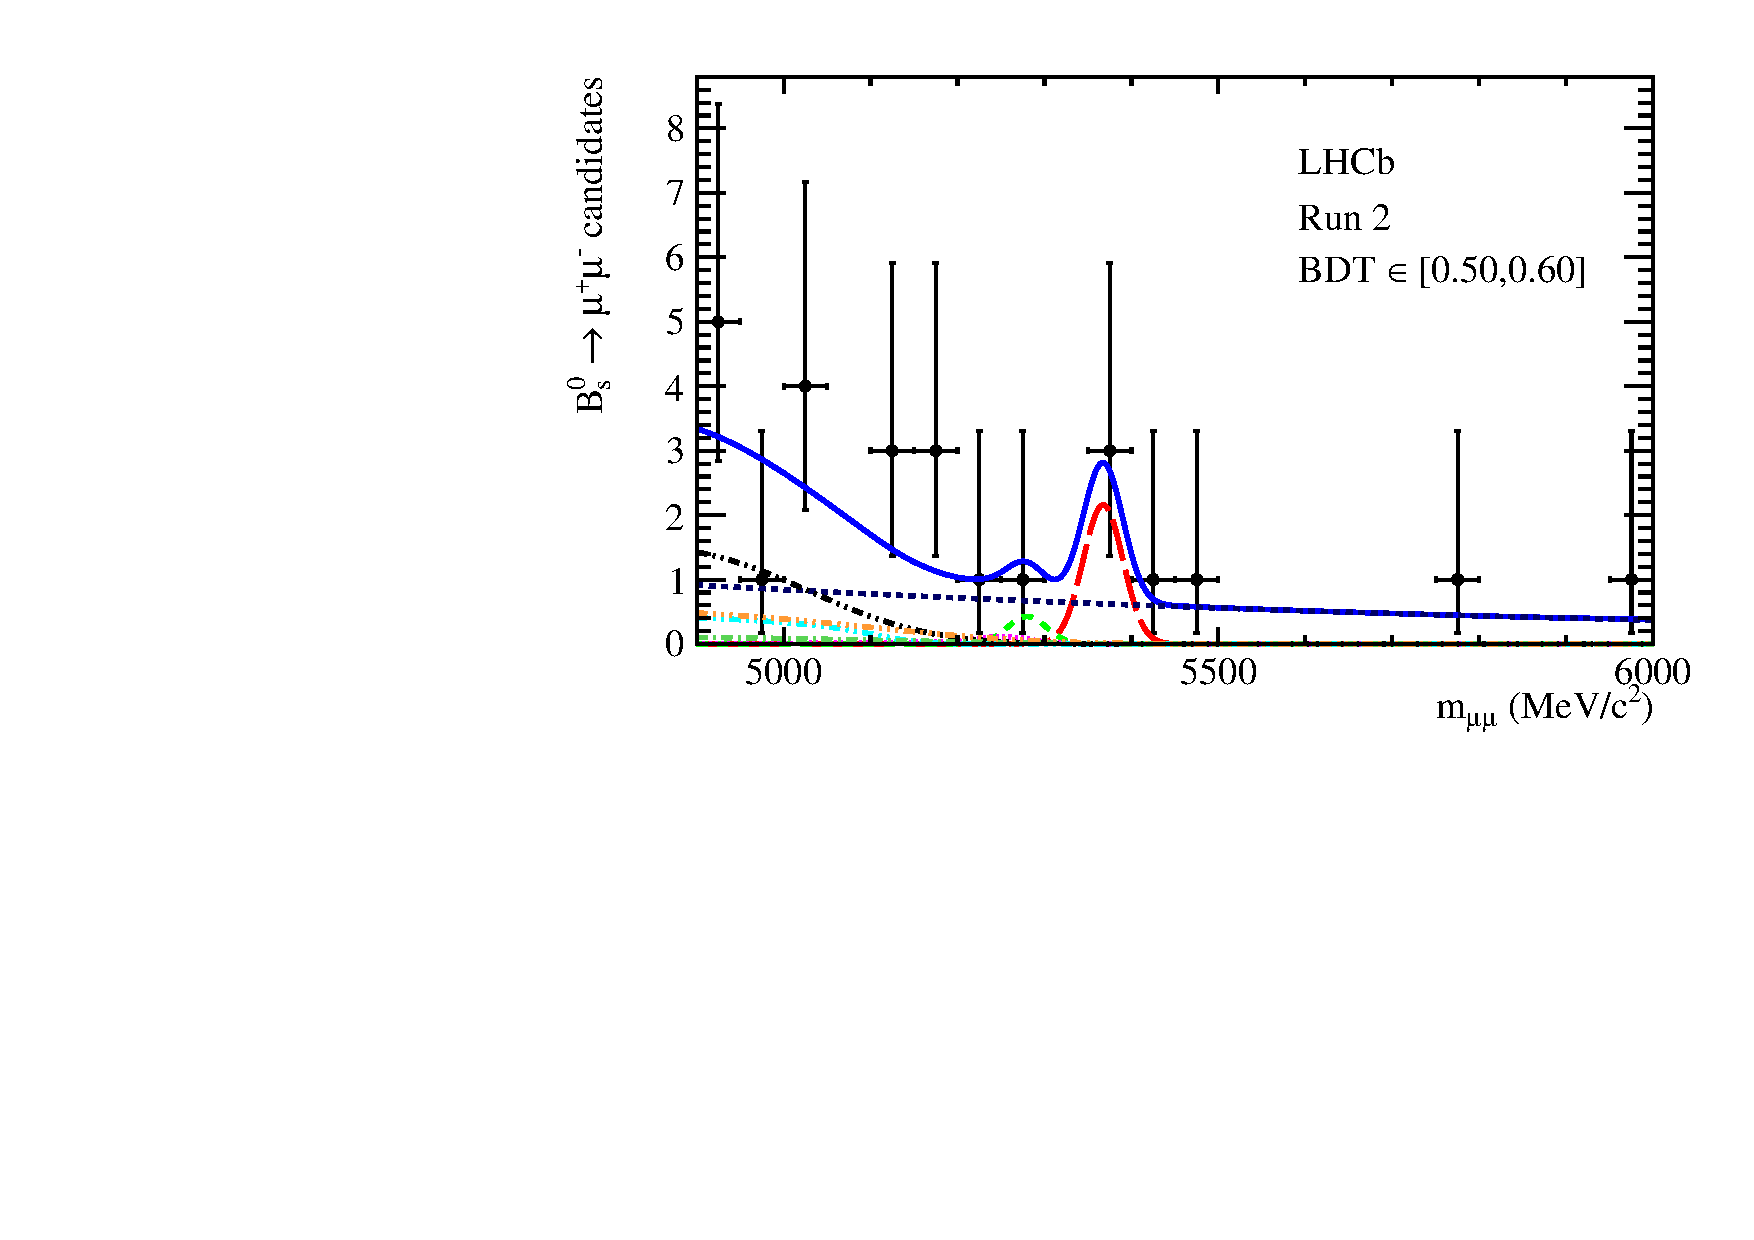
\includegraphics[width=\textwidth]{./Figs/BFAnalysis/Bsmumu_Fit_Run2_bin4.pdf}
    \end{subfigure}
    ~ %add desired spacing between images, e. g. ~, \quad, \qquad, \hfill etc. 
      %(or a blank line to force the subfigure onto a new line)
    \begin{subfigure}[b]{0.48\textwidth}
       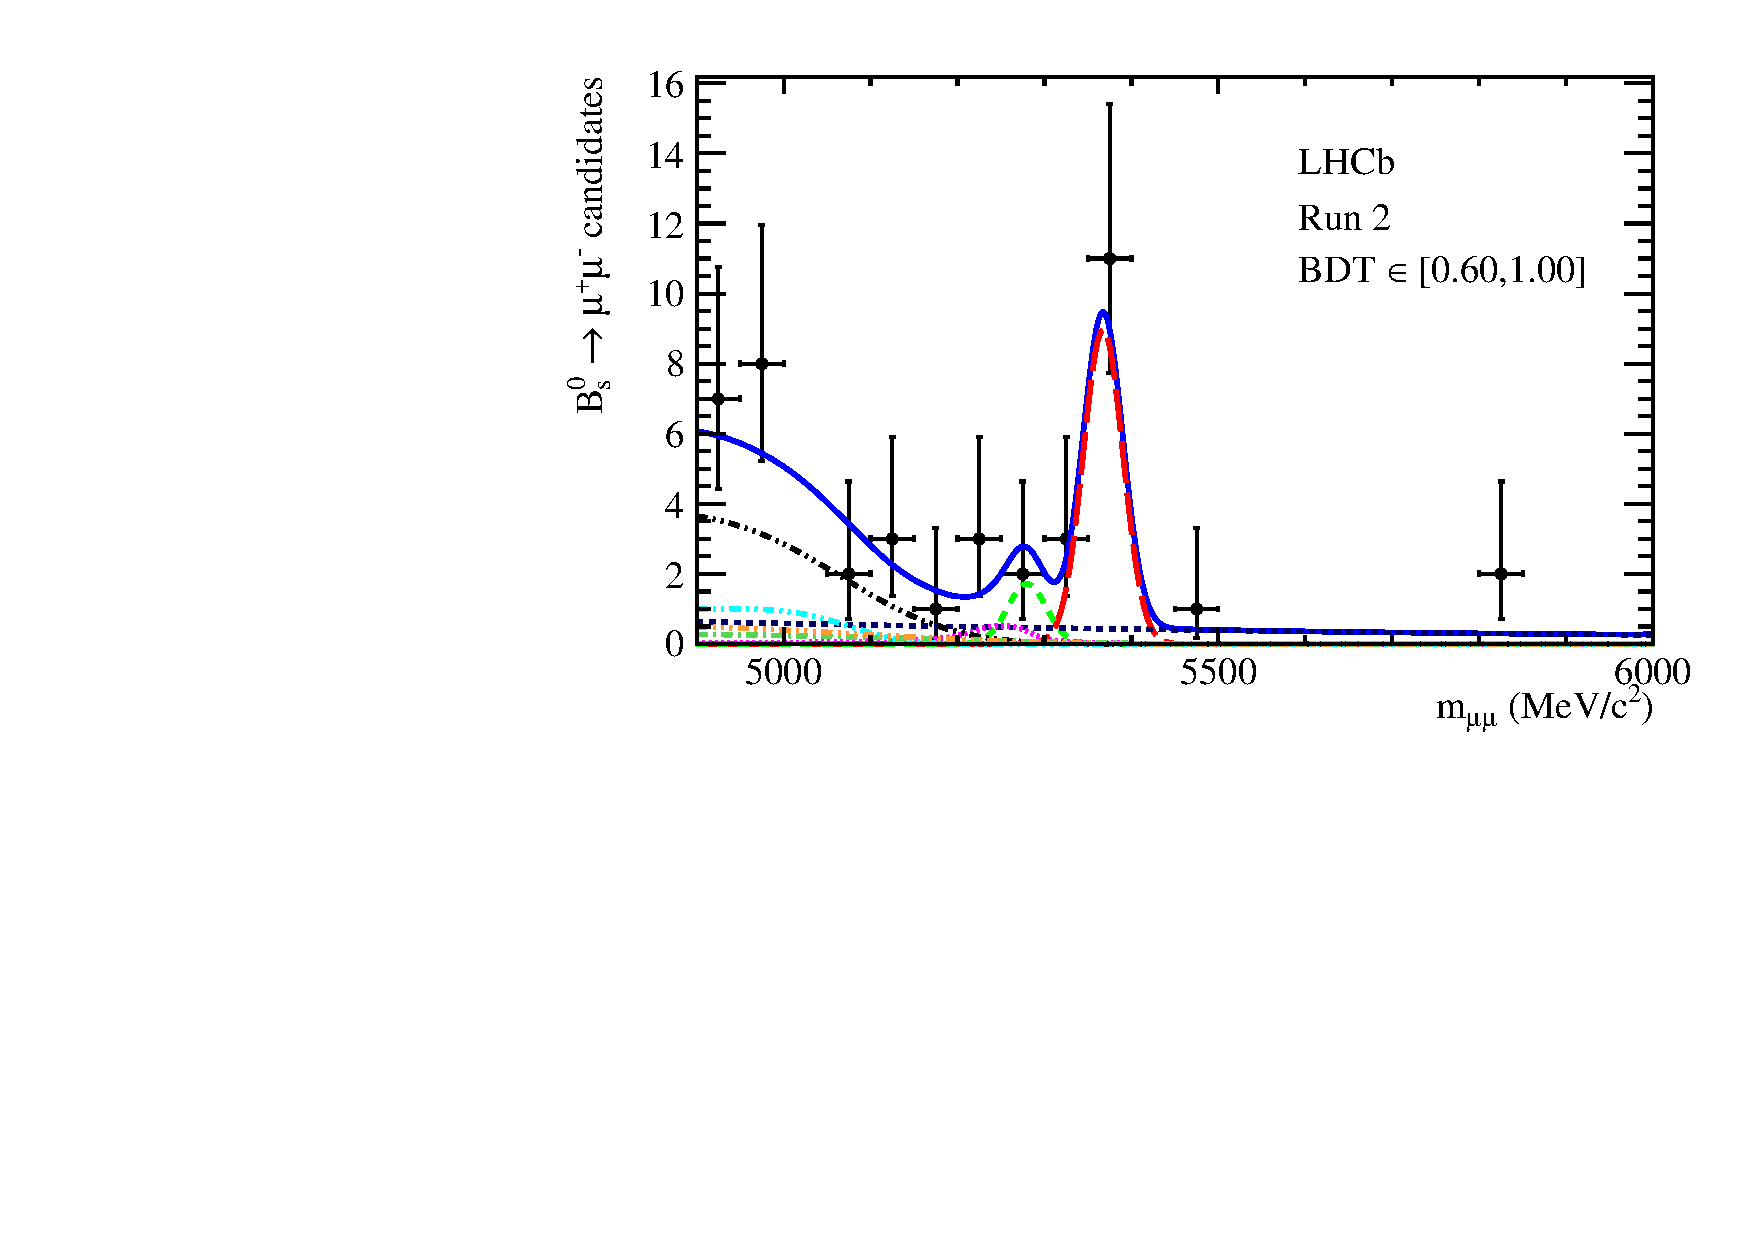
\includegraphics[width=\textwidth]{./Figs/BFAnalysis/Bsmumu_Fit_Run2_bin5.pdf}
    \end{subfigure}

    \begin{subfigure}[b]{0.3\textwidth}
       \includegraphics[width=\textwidth]{./Figs/BFAnalysis/legendB.pdf}
    \end{subfigure}
    ~
    \begin{subfigure}[b]{0.3\textwidth}
       \includegraphics[width=\textwidth]{./Figs/BFAnalysis/LegendA.pdf}
    \end{subfigure}
    \caption{Mass distribution in BDT bins for selected \bsmumu and \bdmumu candidates with the fit overlaid for Run 1 and Run 2 data. The components in the total mass pdf (blue) are; \bsmumu (red), \bdmumu (green), \bhh (magenta), \bdpimunu and \bsKmunu (black), \bcjpsimunu (orange), \bpimumu (cyan), \lambdab (green) and combinatorial background (blue).{\it Think about the key, ideally consistent throughout all images! } }
    \label{fig:BFfit}
\end{figure}



{\bf some things I should learn about the BF anyslsis or I think I should mention. The correlaction, orlack ok, between the mass and BDT output. The cascade B decays that are removed by the lower 4900 mass cut (Alessio) and also the decays that contribute to CBG (Siim).}

{\it prehaps put plots and numbers in the appendix??}
